\documentclass[11pt,a4paper]{article}
\usepackage[margin=2.5cm]{geometry}
\usepackage[T1]{fontenc}
\usepackage{amssymb}
\usepackage{newtxtext,newtxmath}
\usepackage{graphicx}
\usepackage{booktabs}
\usepackage{tabularx}
\usepackage{array}
\usepackage{longtable}
\usepackage{caption}
\usepackage{float}
\usepackage{pdflscape}

\usepackage{enumitem}
\usepackage{amsmath}
\usepackage{xurl}
\usepackage[hidelinks]{hyperref}
\usepackage{microtype}
\captionsetup{font=small,labelfont=bf,skip=4pt}
\setlist{nosep,leftmargin=1.2em}
\setlength{\parskip}{0.35em}
\setlength{\parindent}{0pt}
\renewcommand{\arraystretch}{1.15}
\title{\textbf{Price $\times$ Open-Interest Regimes in Binance Perpetual Futures}\\[4pt]
\large What Positioning Data Does and Does Not Predict}
\author{Sun Yusu\\[2pt]\small Student ID 1155267751\\[6pt]
\small Academic Supervisor: Professor Wu Xixin\\
\small Industrial Supervisor: Mr. Jackson Wong}
\date{27 November 2026}
\begin{document}
\maketitle

\bigskip

\begin{abstract}
Cryptocurrencies’ perpetual futures report open interest data continuously. Quantitative research reads price up with open interest up as fresh long positioning, price up with open interest down as short covering, and the two other quadrants as fresh shorts and long unwinding. This study analyses whether the above four regimes contain pricing and volatility information on the 50 most liquid Binance USDT-M perpetuals between December 2021 and August 2026. Regime membership is attained when the absolute value of hourly price change and open interest change both exceed their respective 90-day 70th percentiles. Regime data (256,079 in total) is analysed using one, four, eight and twenty-four hour ahead returns.

The four regimes distinguish forward volatility clearly. All 16 cell-horizon estimators pass Benjamini--Hochberg correction after two-way clustering, with contract and month effects. Furthermore, following conditioning on funding rate, 83 of the 96 log-volatility contrasts also pass Benjamini--Hochberg correction. Forward direction depends on how the hours are weighted. When counting every event-hour equally, 6 of 16 estimates are significant after BH correction, but when counting every contract-day equally, the sign reverses in all four cells. In our study, no regime clears the 20 bp round trip at any horizon.

A filter of four gates, followed by a mapping step, reduces 96 candidate cells to two arms (section 6.4). Both sit in R4, the regime where price and open interest fall together: A1 holds eight hours at negative funding, B1 one hour at high market volatility. Both lose money over the full sample (net Sharpe $-$0.62 and $-$1.41), and both fail the same way: 10.38 and 9.26 bp of gross edge against a 20 bp round trip. A1 earns 8.79 bp from price and 1.59 bp from funding; B1 earns 9.32 bp from price and pays 0.06 bp in funding. Charged the 20 bp, both are net negative, so neither is tradable.

\end{abstract}
\newpage
\tableofcontents
\newpage
\section{Introduction}

\subsection{Background}

Open interest is the number of contracts opened and not yet closed. It rises when both sides of a trade open a new position, falls when both close, and stays flat when one closes into another's new position. Each contract counts once, so the figure is the size of one side of the book. Volume counts every hand-off; open interest counts only what remains open.

The perpetual never expires, so open interest measures outstanding exposure rather than a schedule of contracts rolling forward. A change in it is the closest public proxy for capital arriving or leaving the book.

Trading commentary has settled on a four-quadrant reading of the pair: price up with open interest up means fresh buying, price up with open interest down means short covering, and the remaining two quadrants mean fresh shorts and long unwinding. That reading is a claim about who is trading now. This study asks whether it is also a claim about what happens next.

\subsection{Problem Statement}

A price move and a change in open interest can occur together, but the pair admits more than one interpretation: open interest may rise because new positions are being opened, or because one side is being replaced by another. The popular four-quadrant reading resolves this ambiguity by assigning intent to each combination. Whether that assignment predicts anything is an empirical question, and the data cannot answer it by inspection.

A significance test on its own would not settle it. Two regimes can differ from each other and still both lose money, so a significant difference is not yet a result. A regime that says how far the next move will go says nothing about which way it goes, and the two are easily confused. And a regime that beats zero may still add nothing: the open-interest layer has to earn its place on top of a price signal that already exists.

The study asks three questions. Does the regime add anything to a rule that uses price alone --- about the direction of the next move, about its size, and about whether the move reverses or continues? Does the funding environment change the answer? And does what survives pay for a round trip? A negative answer to any one of them rejects the claim, and "real but not usable" is a valid outcome here.

\subsection{Scope}

The study covers Binance USDT-M perpetual futures on hourly UTC bars. The panel runs from December 2021 to August 2026; the analysis window is March 2022 to August 2026, because the first three months are needed to warm up the rolling thresholds. Each month the universe is the fifty contracts with the highest 30-day quote volume after four eligibility gates. Returns are measured over one, four, eight and twenty-four hours, and the execution test trades each surviving regime in the direction of its mean at taker cost. Spot, options, dated futures, cross-exchange arbitrage, sub-hourly bars, maker execution and live deployment are out of scope.

\subsection{Motivation}

Open interest is already part of how crypto traders talk about price, but the vocabulary is verbal: a move is "confirmed" or "unconfirmed", positioning is "fresh" or "unwinding". None of it is measured, and two readings can conflict without either being wrong. A framework that fixes the labels, the thresholds and the horizon turns the argument into something that can be checked, priced and monitored.

The appeal is partly practical. The inputs are public, free and hourly, the costs are known, and the same pipeline can rerun on a new venue or a new year. If the directional part does not survive execution, what remains still earns its place: a variable that says how volatile the next few hours are likely to be, and a board that shows each liquid contract's regime and where the market sits.

\subsection{Expected Outcome}

A clean pipeline: Binance public data for price, open interest, funding and volume, stored as parquet with a data dictionary.

A four-regime classifier with explicit thresholds.

An event study measuring forward return at one, four, eight and twenty-four hours, reversal against continuation, the funding interaction, volatility, and path outcomes (maximum favourable and adverse excursion, drawdown), each against four baselines: price alone, open interest alone, funding alone, random timing.

A strategy prototype of one or two rules, costed and compared with those same baselines.

A board showing the current regime of each contract, fresh long and short buildups, deleveraging candidates and funding-adjusted crowding.

\bigskip

\section{Literature Review}

\subsection{Positioning data as an information source}

Two arguments support treating positioning as information. One is that it anticipates returns. The other is that a perpetual publishes what a position costs to hold: the funding rate one side pays the other, which moves with the balance of positioning.

Seo, Byun and Kim (2020) give the cleanest equity-side evidence. Growth in out-of-the-money index call open interest forecasts subsequent stock-market returns, and the effect survives controls for volume and past returns. The direction of that result matters here: positioning leads, price follows, and the mechanism is informational rather than mechanical.

The perpetual makes the same test possible at hourly frequency and adds a measurement problem. Giagkiozis and Said (2024) reconcile open interest with traded volume in perpetual swaps and find systematic discrepancies at some large venues, so an open-interest change read from one venue may not describe the same population as the price printed beside it. Every four-quadrant study inherits that bias, our study included.

Funding is what a perpetual has instead of an expiry date. He, Manela, Ross and von Wachter (2022) show how loose that anchor is: crypto perpetuals drift from spot, the drift is common across coins and decays, and the gap is wide enough to arbitrage. None of this is about open interest directly. What it establishes is where the cost of holding a position shows up, and that is why funding enters here as a second dimension of the analysis rather than as a rival predictor.

Kim (2026) tests the second argument directly. HAR forecasts of Bitcoin spot volatility improve with funding-rate measures both in and out of sample, with gains at weekly and monthly horizons. Open-interest change alone is not significant; its interaction with funding is, at 0.661 weekly (t = 2.70) and 0.393 monthly (t = 2.41). Kim reads the mechanism as imbalanced leveraged positions unwinding over days. His sample is Bitcoin, at daily frequency and coarser, so it does not answer the cross-sectional hourly question asked here. It does show that positioning carries information about volatility, and that open interest carries it in combination rather than alone.

\subsection{Momentum, reversal and the horizon}

Zaremba et al. (2021) test more than 3,600 coins and find that the previous day's return reverses on average, while the largest and most tradeable coins show daily momentum. The payoff of a price-only rule therefore depends on the universe and on the horizon, which is why it has to be rebuilt here rather than imported.

In our study, Phase 3 rebuilds that rule on exactly the same events: long when price is up past its threshold, short when it is down, open interest ignored. On the top fifty at hourly frequency it earns $-$1.43 bp at one hour and stays negative at the longer horizons. Momentum in liquid coins turns out to be a daily phenomenon that does not reach the hourly grid.

Naredla (2026) is the closest precedent to our study in design. Using perpetual basis and hourly funding as state coordinates for regime detection, he finds that they beat hidden-Markov and rolling-volatility baselines on forward-volatility regimes by five to seven percentage points, while failing to predict sub-daily direction. The shape of the result is the same with different state variables, and it is the strongest prior that the volatility finding in Section 6.1 is not an artefact.

\subsection{Costs and the distance between a signal and a strategy}

Jadouli (2026) is the closest to our study in results, and it is a negative result. Candle-based timing models on Binance spot rank the next move well, with ROC-AUC of 0.874 and 0.896, and select badly: average precision of 0.134 and 0.116, and $-$44.3\% over seven cycles against $-$41.2\% for buy-and-hold. The gross advantages it measures elsewhere, 11.11 and 12.21 bp per cycle, sit below the paper's 21 bp stress cost. Ranking skill is not equal to profit.

None of the cost figures in Section 4.6 are estimated. Brauneis et al. (2021) show that crypto spreads can be estimated and identify which estimators do it best: Corwin-Schultz and Abdi-Ranaldo for high-frequency spreads, Kyle-Obizhaeva and Amihud for levels and venue differences. This study assumes a 20 bp taker round trip, then reports a break-even cost for every arm, so a reader with a better estimate can re-price the result.

Volatility forecasting has a benchmark this study does not try to meet. Christensen, Siggaard and Veliyev (2023) show that machine-learning models beat HAR for realised variance even when restricted to lagged realised variance, with gains that grow with horizon. Section 6.1 does not compete on forecast accuracy. Instead, it reports a difference in the conditional mean of realised volatility across regimes, which is not a forecasting model.

\subsection{Inference discipline}

Two problems arise when one sample is asked many questions: some tests will look significant by chance, and standard errors that ignore shared shocks will be too small.

Harvey and Liu (2020) show that the 1.96 cutoff is too loose in finance, where hundreds of relations are tested. Hou, Xue and Zhang (2020) find that 82\% of 452 published anomalies fail a stricter 2.78. Jensen, Kelly and Pedersen (2023) find that most published factors do replicate, so the stricter cutoff also discards real findings. This study applies Benjamini--Hochberg at five per cent inside a family declared at each stage, and reports every result in that family after the correction.

The standard errors follow Cameron, Gelbach and Miller (2011) and Petersen (2009): two-way clustering on contract and calendar month, because observations sharing either are not independent.

\subsection{What this study adds}

This study holds the three together on a monthly top-fifty universe drawn from 249 contracts, at hourly frequency. Volatility separates cleanly: all 16 regime-by-horizon estimators survive BH correction. The price--open-interest interaction, meaning whether the effect of open interest depends on the direction of price, is significant at every horizon, with t-statistics from 2.8 to 4.3. Two things fail. The sign of the directional effect changes with the weighting, and the two states that clear the gates earn only about 10 bp gross, which turns negative once the 20 bp round trip is charged.

\section{Market Research}

\subsection{Market structure}

A USDT-M perpetual is a margined derivative that tracks a spot index and never expires. Two institutional features matter for this study.

The first is funding. Longs and shorts exchange a payment at an interval the exchange sets per contract, sized to pull the perpetual toward the index. The interval is not constant across the sample: almost every settlement was eight-hourly in 2022, and 73\% were four-hourly by 2026. Funding is a public price of positioning --- when the perp trades above spot, longs pay --- and it does not depend on open interest, which is why it enters as a conditioning variable rather than as a separate signal.

The second is disclosure. Open interest is published per contract on the same hourly grid as price, with no aggregation across venues, so an event window and its price path line up without interpolation. It is a snapshot series rather than a tick feed: the historical endpoint's finest interval is five minutes, and this study archives hourly.

\subsection{Why this market suits the question}

Four properties make the test unusually clean. Trading is continuous, so there is no overnight gap between the signal and the entry. Open interest, price and funding are printed by one exchange at one timestamp, which rules out an aggregated cross-venue tape. There are no price limits, so a large move is not truncated by an exchange rule. And the contract set is large enough that a monthly top-fifty universe can be rebuilt from public data alone, which is what makes the result reproducible.

\subsection{Concentration and churn}

Trading is concentrated. A median of 182 contracts change hands in a month, and the fifty largest carry 85\% of the volume. The rest are thin enough that a fill assumption built on them would not survive contact with the book, which is why the universe stops at fifty.

Membership of that fifty turns over. Around eight contracts leave each month and eight arrive, about 16\% of the list. Across the fifty-four months there are 446 replacements. The median contract in the panel lives just under three years, and 12\% live less than one year. A universe fixed at the end of the sample would keep only the survivors, which is why this one is rebuilt every month and Section 4.1 sets out how.

\bigskip

\section{Methodology}

\subsection{Data}

The sample is every USDT-M perpetual contract listed on Binance between 2021-12-01 and 2026-08-31, at hourly frequency, in UTC. The start date is not a design choice: the archived open-interest series begins there, and an earlier start would leave the OI side empty.

The panel is a dense hourly grid. Every hour between a contract's first and last bar has exactly one row, and missing hours are retained with bar\_missing and oi\_missing flags. The row count is therefore the size of the grid, not the number of observations: 7,253,002 rows for 285 contracts over 57 months. Treating grid rows as observations would overstate effective sample size, so every count reported later is conditional on ok\_h, the flag that requires a valid forward window.

\textbf{Universe construction.} Each month, contracts are ranked by 30-day quote volume and the top fifty kept, after four gates: stablecoin and fiat bases excluded (a hand-maintained list of eleven, since no single exchange label covers them); at least 2,160 prior hourly bars and still trading at the start of the month, the second condition because a delisted contract's bar count freezes and LUNAUSDT would otherwise pass for ever; open-interest coverage of at least 90\% over the trailing 30 days with no publication gap longer than 48 hours, counted on different denominators because the first treats a missing hour as a failure and the second deliberately ignores hours where the price grid is absent; and tokenised equities, ETFs and currencies excluded, so that only crypto perpetuals enter, with PAXG and XAUT kept because they trade around the clock. What remains is truncated at fifty by the median quote volume of the same thirty days.

This produces 2,700 contract-month cells covering 249 contracts over 54 membership months. The first three months of the sample have an empty universe, because no contract yet has ninety days of history, which is why the panel spans 57 months while membership spans 54.

Rebuilding the universe every month is what controls survivorship. A contract contributes to the months in which it was in the top fifty, including months that precede its delisting, and stops contributing after that. No contract is dropped for having failed later, and none is kept for having succeeded. The 446 replacements in Section 3.3 give the size of the problem: a universe fixed at the end of the sample would contain only the contracts that survived all of it.

\subsection{Regime construction}

For each contract-hour the one-hour price change is $\Delta$p = close\_t / close\_\{t$-$1\} $-$ 1, and the open-interest change is computed over the same interval. Both thresholds are the 70th percentile of the absolute change over the contract's own trailing ninety calendar days, with at least thirty days of history required before a threshold is issued.

A contract-hour becomes an event when both absolute changes exceed their thresholds. The quadrant then follows from the signs:

\begin{table}[H]\centering
\footnotesize
\begin{tabularx}{\linewidth}{>{\raggedright\arraybackslash}X>{\raggedright\arraybackslash}X>{\raggedright\arraybackslash}X>{\raggedright\arraybackslash}X}
\toprule
Cell & Price & Open interest & Retail reading \\
\midrule
R1 & up & up & fresh longs \\
R2 & up & down & short covering \\
R3 & down & up & fresh shorts \\
R4 & down & down & long unwinding \\
\bottomrule
\end{tabularx}
\end{table}

Two properties decide how the results should be read. The threshold is on the absolute change, so an event means a large move rather than a directional trend. And the label is an hourly event flag attached to the bar at which the threshold was crossed, not a persistent state: 12.7\% of contract-hours sit in one of the four cells, and at any single hour only a handful of the fifty contracts qualify.

The funding dimension is separate. Each contract's rate is labelled against its own rolling distribution --- below the 25th percentile is negative, above the 75th is high --- so a label describes how unusual the rate is for that contract, not how expensive the position is in annual terms. Settlement intervals shortened over the sample, from eight hours to four for most contracts, and these quantiles follow within a few months of the change.

\subsection{Data and label quality}

The panel is not clean, and the places where it is not clean are known. Seven of the fifty-seven months contain a day on which at least a fifth of live contracts lack one of the four sources: two are holes in the klines archive, four are exchange-wide outages (one of them index-only, on 31 July 2022), and one is an exchange-wide open-interest gap on 16 February 2024 that leaves 58\% of contracts without it. None of these is patched by interpolation. They are excluded by the universe gates instead, which require 90\% open-interest coverage over the trailing thirty days with no gap longer than 48 hours, so a contract-month containing a hole drops out rather than entering with a filled value.

\begin{figure}[H]
\centering
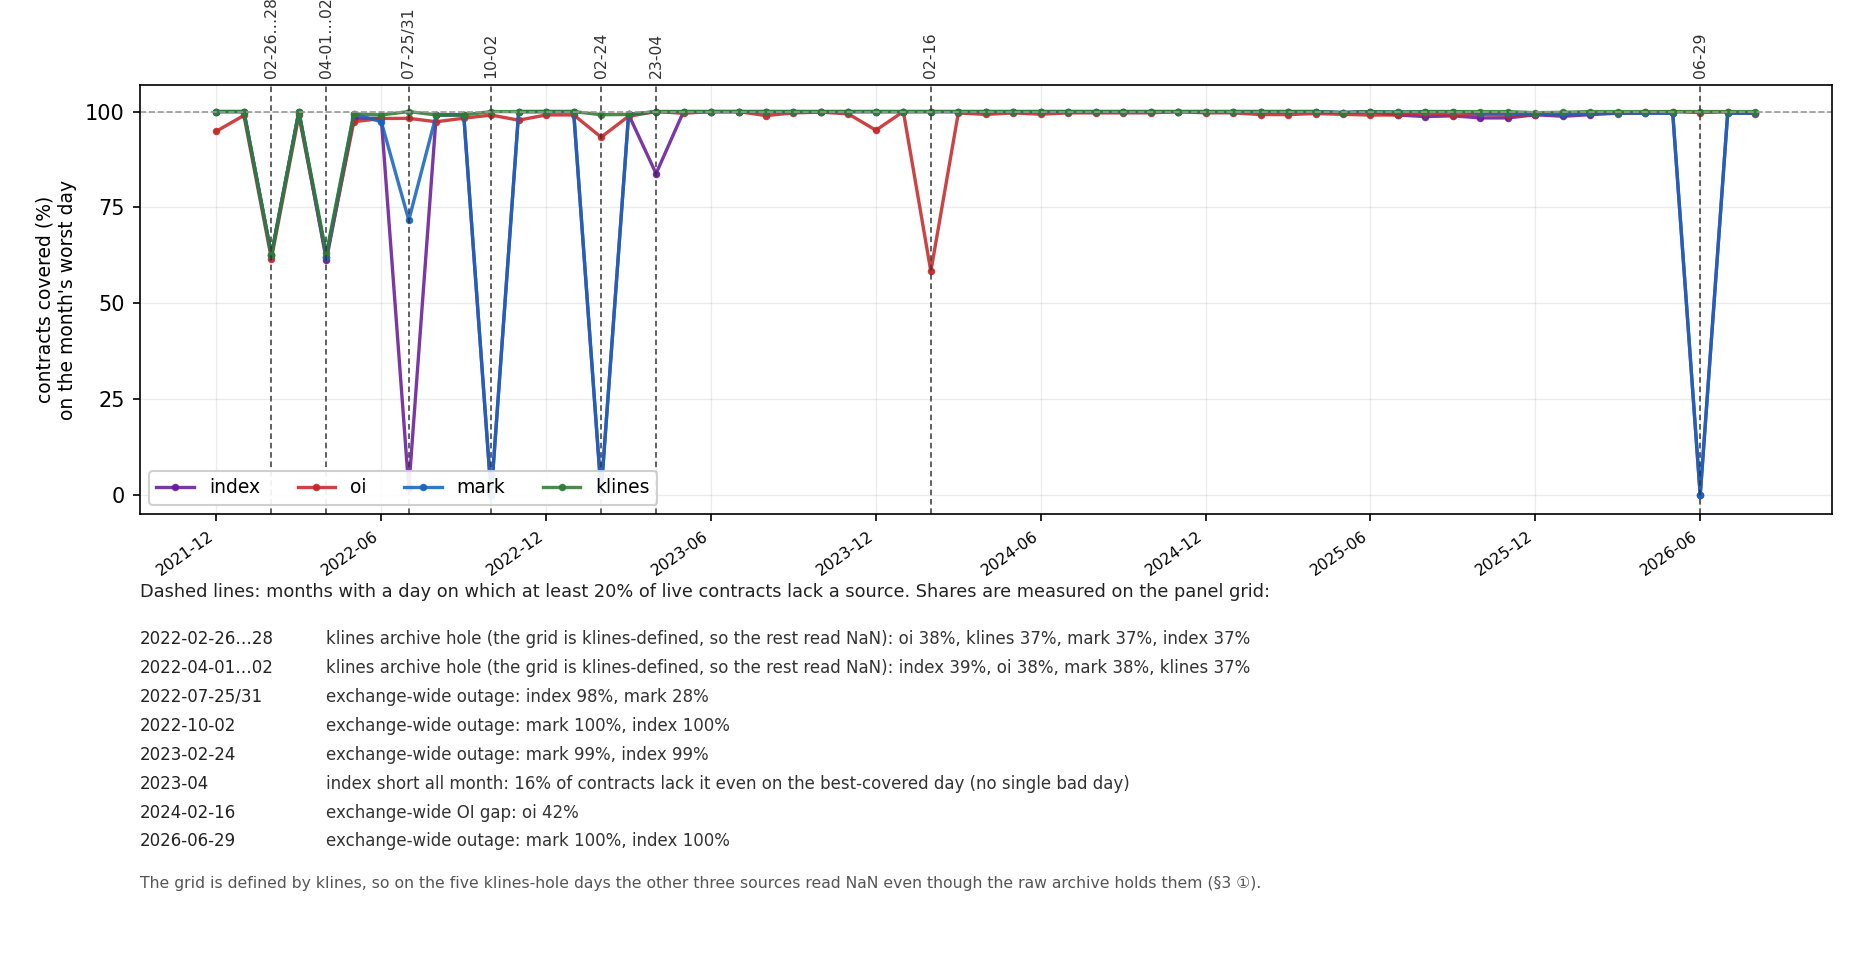
\includegraphics[width=0.92\linewidth,height=0.40\textheight,keepaspectratio]{figs/q1_coverage.png}
\caption{Coverage by month, 2021-12 to 2026-08. A point is the share of contracts covered by that source on the month's worst day; dashed months contain a day on which at least 20\% of live contracts lack a source, and the footnote lists the cause of each.}
\end{figure}

The labels have one free parameter, the threshold, and it is worth knowing what it is worth. Moving the cut from the 55th to the 80th percentile lowers the labelling rate from 23.0\% to 7.5\%, which is mechanical: a stricter cut labels fewer hours. What matters is the mix. Within the labelled set the four quadrants keep their relative shares, with a largest move of 3.8 pp at one hour and 11.8 pp at one day. Section 6 is therefore about a p70 choice that could have been p60 or p80 without changing which quadrant is which.

\begin{figure}[H]
\centering
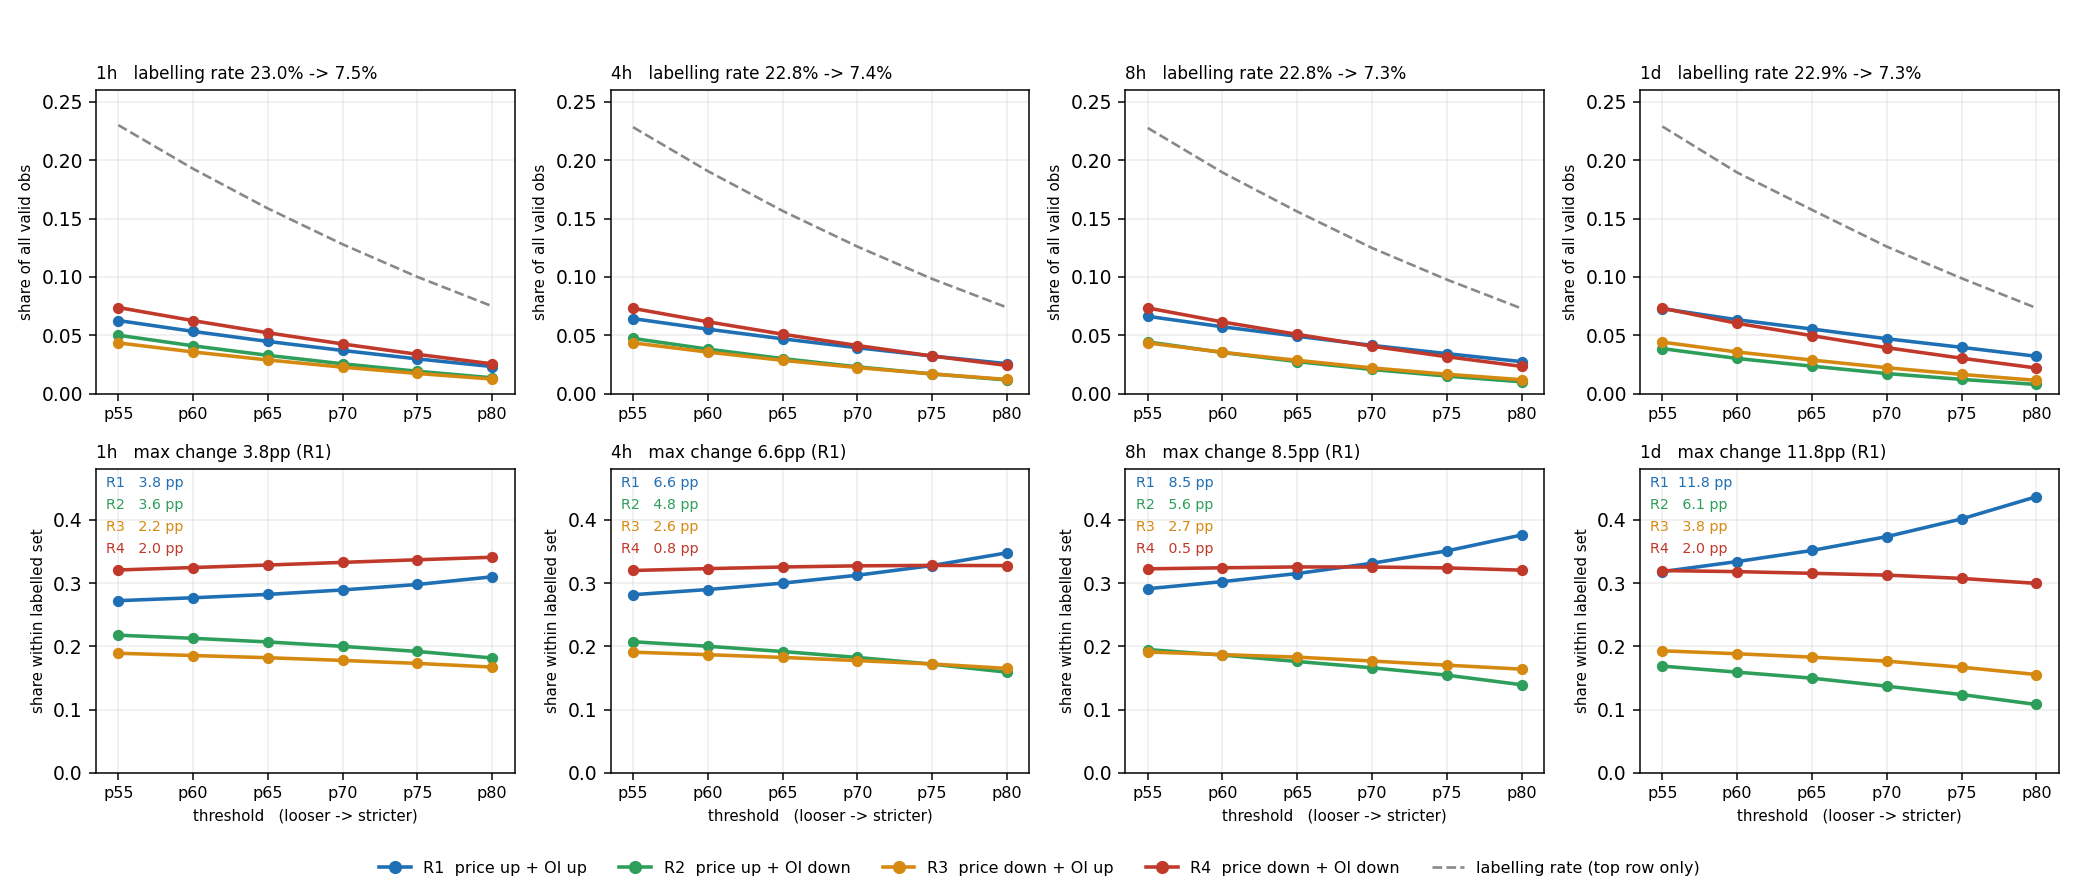
\includegraphics[width=0.92\linewidth,height=0.40\textheight,keepaspectratio]{figs/q2_threshold.png}
\caption{Threshold sensitivity. Top row: each label as a share of all valid observations, dominated by the fall in the labelling rate. Bottom row: each label as a share of the labelled set, so the four sum to 100\% at every point; the largest move over the six thresholds is printed in each panel.}
\end{figure}

\subsection{Event study: what each experiment tests}

Forward returns are close-to-close over 1, 4, 8 and 24 hours. Each is reported twice: raw, and net of the same-hour mean across the whole labelled pool, not only the contracts in the universe. The second quantity, written y\_raw and called the market-neutral return below, is therefore the forward return minus the same-hour market-wide mean. That cross-section holds 174 contracts an hour across 41,639 labelled hours, and y\_raw is the quantity that carries any claim about alpha. Three objects recur and are not interchangeable: the raw forward return, the market-neutral return y\_raw just defined, and the increment, which is the regression coefficient against the same-direction benchmark and therefore a difference between a cell and its benchmark rather than a level.

Estimation is a fixed-effects regression of the forward return on the regime indicator, with contract and month effects, so the coefficient is the regime less its same-direction benchmark. Standard errors are two-way clustered on contract and calendar month (Cameron, Gelbach and Miller, 2011; Petersen, 2009), for the reason set out in Section 2.4. The event-study tests are two-sided on the mean against the same-direction benchmark. The gate in Section 4.6 is two-sided, because there the sign of the mean also chooses the side of the trade.

Eight experiments carry a test, and they run in the order Phase 3 specified them:

\begin{table}[H]\centering
\footnotesize
\begin{tabularx}{\linewidth}{>{\raggedright\arraybackslash}X>{\raggedright\arraybackslash}X>{\raggedright\arraybackslash}X}
\toprule
\# & Question & Measured as \\
\midrule
1 & Do regimes differ from a price-only benchmark? & Forward return minus the same-direction benchmark, with contract and month effects \\
1b & Does the effect of open interest depend on the direction of price? & Open-interest increment at fixed price direction, price increment at fixed OI direction, and the interaction of the two \\
3 & Do regimes separate future volatility? & Forward realised volatility against the same benchmark \\
4 & Does the move continue or reverse? & Reversal probability against the same-direction benchmark \\
5--7 & Can price, open interest or funding alone do the work? & Each single-signal spread against zero \\
8 & Is the timing arbitrary? & Regime return against 1,000 random-time draws per contract \\
9 & Does the four-state spread beat the three baselines? & Twelve gaps, with the random-timing result as a fourth reference \\
15 & Does it hold when one vote is given per contract-day? & The same events reweighted \\
\bottomrule
\end{tabularx}
\end{table}

Two items are numbered but carry no test. Experiment 2 puts the median beside the mean, as a check that the mean is not the work of a few large trades. Experiments 10 to 14 are descriptive tables: cell levels (10), path measures (11), hourly event paths (12), the four baselines as levels (13), and the by-coin and by-market-state splits (14). Section 6 reports them, and no claim rests on them alone.

Multiplicity is controlled by Benjamini--Hochberg at q < 0.05 within a family declared per experiment: sixteen for the four-cell by four-horizon designs, twenty for the factor decomposition, twenty-eight across experiments 5 to 9, and sixteen for the reweighted run.

\subsection{Conditioning on funding}

Phase 3 tests funding once, as a standalone baseline (experiment 7). Phase 4 makes it a dimension of the same event. Each regime is re-estimated inside each funding state, so the question becomes whether a regime survives a given cost of carry rather than whether funding predicts on its own. The states are cut on the contract's own trailing 90-day settlements: negative at or below the 25th percentile, neutral to the 75th, high above it, extreme above the 90th. They are nested rather than partitioned, every regime still contains all four, and a cell is the same regime under a different funding label.

Seven blocks make up Phase 4, and they run in this order:

\begin{table}[H]\centering
\footnotesize
\begin{tabularx}{\linewidth}{>{\raggedright\arraybackslash}X>{\raggedright\arraybackslash}X>{\raggedright\arraybackslash}X>{\raggedright\arraybackslash}X}
\toprule
ID & Question & Measured as & Family \\
\midrule
P4-1 & Does the return of a regime depend on the funding state? & Twelve within-regime contrasts, each funding level against neutral & 12 per weighting and horizon \\
P4-2 & Does the volatility result depend on it as well? & Realised volatility levels and log changes, on the same twelve contrasts & 12 \\
P4-3 & Does the continuation or reversal probability shift? & Linear probability model of reversal and continuation & 12 \\
P4-4 & What does the path inside a cell look like? & Maximum favourable and adverse excursion, drawdown & descriptive \\
P4-5 & Is the regime effect a beta to the benchmark? & Regime and benchmark coefficients on the same two outcomes & 16 \\
P4-6 & Does R4 recover faster in some volatility states? & R4 only, split by market-volatility state: mean, reversal share, median drawdown & descriptive, not a test of recovery speed \\
P4-7 & Are high and extreme the same rows? & The same cells recounted on a five-way split, with high-only, extreme and degenerate kept apart, at both weightings & descriptive \\
\bottomrule
\end{tabularx}
\end{table}

Each family is declared per weighting and horizon, and the two weightings are reported side by side, one vote per event and one vote per contract-day, because the choice between them is not innocent. P4-7 checks the labels rather than the results. In most rows the 90th percentile equals the 75th, so high and extreme are then the same rows. The block separates high-only from extreme, labels the remainder degenerate, and recounts the same cells on that five-way split. It carries no test of its own. The beta block is reported but not used as a result: of 384 estimates 72 survive, and the event and contract-day versions differ in sign in several cells.

\subsection{From regimes to strategies}

A contrast compares two cell means. A level is what a position in one cell earns. The two can point in opposite directions. R3 with negative funding has the largest contrast that survives correction, +5.29 bp per hour, against a market-neutral level of +5.56 bp: the contrast is real and the position is still too small to pay for a round trip.

A surviving cell maps to one rule: enter at the open of the first bar within two hours of the event, and exit at the close h hours after entry, or at the last available close if the contract stops printing. Each signal is 2\% of the equity at entry, and gross exposure cannot exceed that capital, so at most fifty positions are open at once. A contract holds one position; a signal that arrives while it is open is dropped. Cost is 20 bp per round trip, 10 bp on entry and 10 bp on exit, and every strategy reports its break-even cost.

The gate has three parts: G0 fixes the input, G1 to G4 are the filters, and G5 turns a survivor into an arm. All of them judge the level rather than the contrast, for the reason above, and only G1 is a statistical test; the rest are sign checks on point estimates.

\begin{itemize}
\item \textbf{G0, input.} Universe, cell and funding state are already fixed by the base; a level is the raw forward return in basis points.
\item \textbf{G1, existence.} Is the level different from zero? Two-sided t, CGM errors, BH over the twelve cells at that horizon, at least 400 events. Its sign sets the side of the trade.
\item \textbf{G2, market.} Is the market-neutral mean on that side, so the level is not beta?
\item \textbf{G3, tails.} Are the median and the mean with 1\% trimmed from each tail on the same side as the trade, so the level is not a few large trades?
\item \textbf{G4, stability.} Is the level on that side in four of the five calendar years and in the trailing twelve months?
\item \textbf{G5, mapping.} One survivor, one strategy, at its own horizon.
\end{itemize}

The order matters. G1 removes most candidates cheaply. G2 and G3 remove the two ways a level can look real without being real, beta and a handful of large trades. G4 removes strategies that exist only in part of the sample.

\bigskip

\section{Proposed Solution}

\subsection{Functional requirements}

The system had to satisfy six requirements, each traceable to a deliverable in the industry brief:

\begin{table}[H]\centering
\footnotesize
\begin{tabularx}{\linewidth}{>{\raggedright\arraybackslash}X>{\raggedright\arraybackslash}X>{\raggedright\arraybackslash}X}
\toprule
ID & Requirement & Delivered by \\
\midrule
FR1 & Ingest and validate exchange data into a reproducible hourly panel & Phase 1 \\
FR2 & Classify each contract-hour into one of four price/OI regimes & Phase 2 \\
FR3 & Measure forward returns, volatility and path outcomes by regime & Phase 3 \\
FR4 & Condition the regimes on funding and test interactions & Phase 4 \\
FR5 & Convert surviving regimes into executable rules and price them & Phase 5 \\
FR6 & Expose the current state of the universe interactively & D5 board \\
\bottomrule
\end{tabularx}
\end{table}

\subsection{Functional design}

Two design choices carry the rest. The first is the unit of analysis: one row per contract-hour, carrying the state knowable at that hour and the outcomes that follow it in separate columns, so a label is always computed from the past and never from the window it is meant to predict. The second is that the comparison lives inside the sample. The price-only benchmark is rebuilt on the same events rather than imported from another study, the market-neutral adjustment uses the same-hour cross-section, and the only number brought in from outside is the cost, which is why every table reports a break-even cost beside it.

\subsection{System architecture}

Everything runs from \texttt{config.py}, which holds every path, threshold and window, and \texttt{lib/\allowbreak{}schema.py}, which declares the type and unit of every column. Five stage directories then read the layer before them and write one data directory each:

\begin{table}[H]\centering
\footnotesize
\begin{tabularx}{\linewidth}{>{\raggedright\arraybackslash}X>{\raggedright\arraybackslash}X>{\raggedright\arraybackslash}X}
\toprule
Stage & Modules & Writes \\
\midrule
\texttt{phase1/\allowbreak{}} & \texttt{fetch\_market\_data}, \texttt{build\_candidate\_pool}, \texttt{build\_layer2}, \texttt{build\_features}, \texttt{build\_universe}, \texttt{build\_deliverables}, \texttt{run\_phase1} & \texttt{data/\allowbreak{}raw}, \texttt{00\_config}, \texttt{01\_layer2}, \texttt{02\_features}, \texttt{03\_reference}, \texttt{04\_qa} \\
\texttt{phase2\_regime/\allowbreak{}} & \texttt{regime\_generator}, \texttt{build\_sensitivity} & \texttt{data/\allowbreak{}05\_regime} \\
\texttt{phase3\_event/\allowbreak{}} & \texttt{build}, \texttt{infer}, \texttt{figures}, \texttt{experiment/\allowbreak{}} & \texttt{data/\allowbreak{}06\_event\_study} \\
\texttt{phase4\_funding/\allowbreak{}} & \texttt{build}, \texttt{figures} & \texttt{data/\allowbreak{}07\_funding} \\
\texttt{phase5\_simple\_strategy/\allowbreak{}} & \texttt{gate}, \texttt{rules}, \texttt{backtest}, \texttt{eval}, \texttt{report}, \texttt{figures}, \texttt{selftest}, \texttt{build} & \texttt{data/\allowbreak{}08\_strategy} \\
\texttt{d5\_dashboard/\allowbreak{}} & \texttt{payload}, \texttt{html}, \texttt{build} & \texttt{data/\allowbreak{}09\_dashboard/\allowbreak{}dashboard.html} \\
\bottomrule
\end{tabularx}
\end{table}

% [TIKZ placeholder removed from the compiled report]
Each stage writes only its own data directory and reads the ones before it, so rerunning a phase cannot rewrite another phase's output, and the board is built from the frozen tables rather than from live code.

\subsection{The dashboard}

The board is one page showing the fifty contracts in the universe at a chosen hour. A selector sets the hour, and each row carries the regime label at that hour together with the most recent event inside the previous twenty-four hours; because a regime is an event flag, the instantaneous label is empty most of the time, so both are shown. The file is a single HTML with the data compressed and embedded, which lets it open from disk without a server; the screenshots in Appendix C are renders of it.

\begin{figure}[H]
\centering
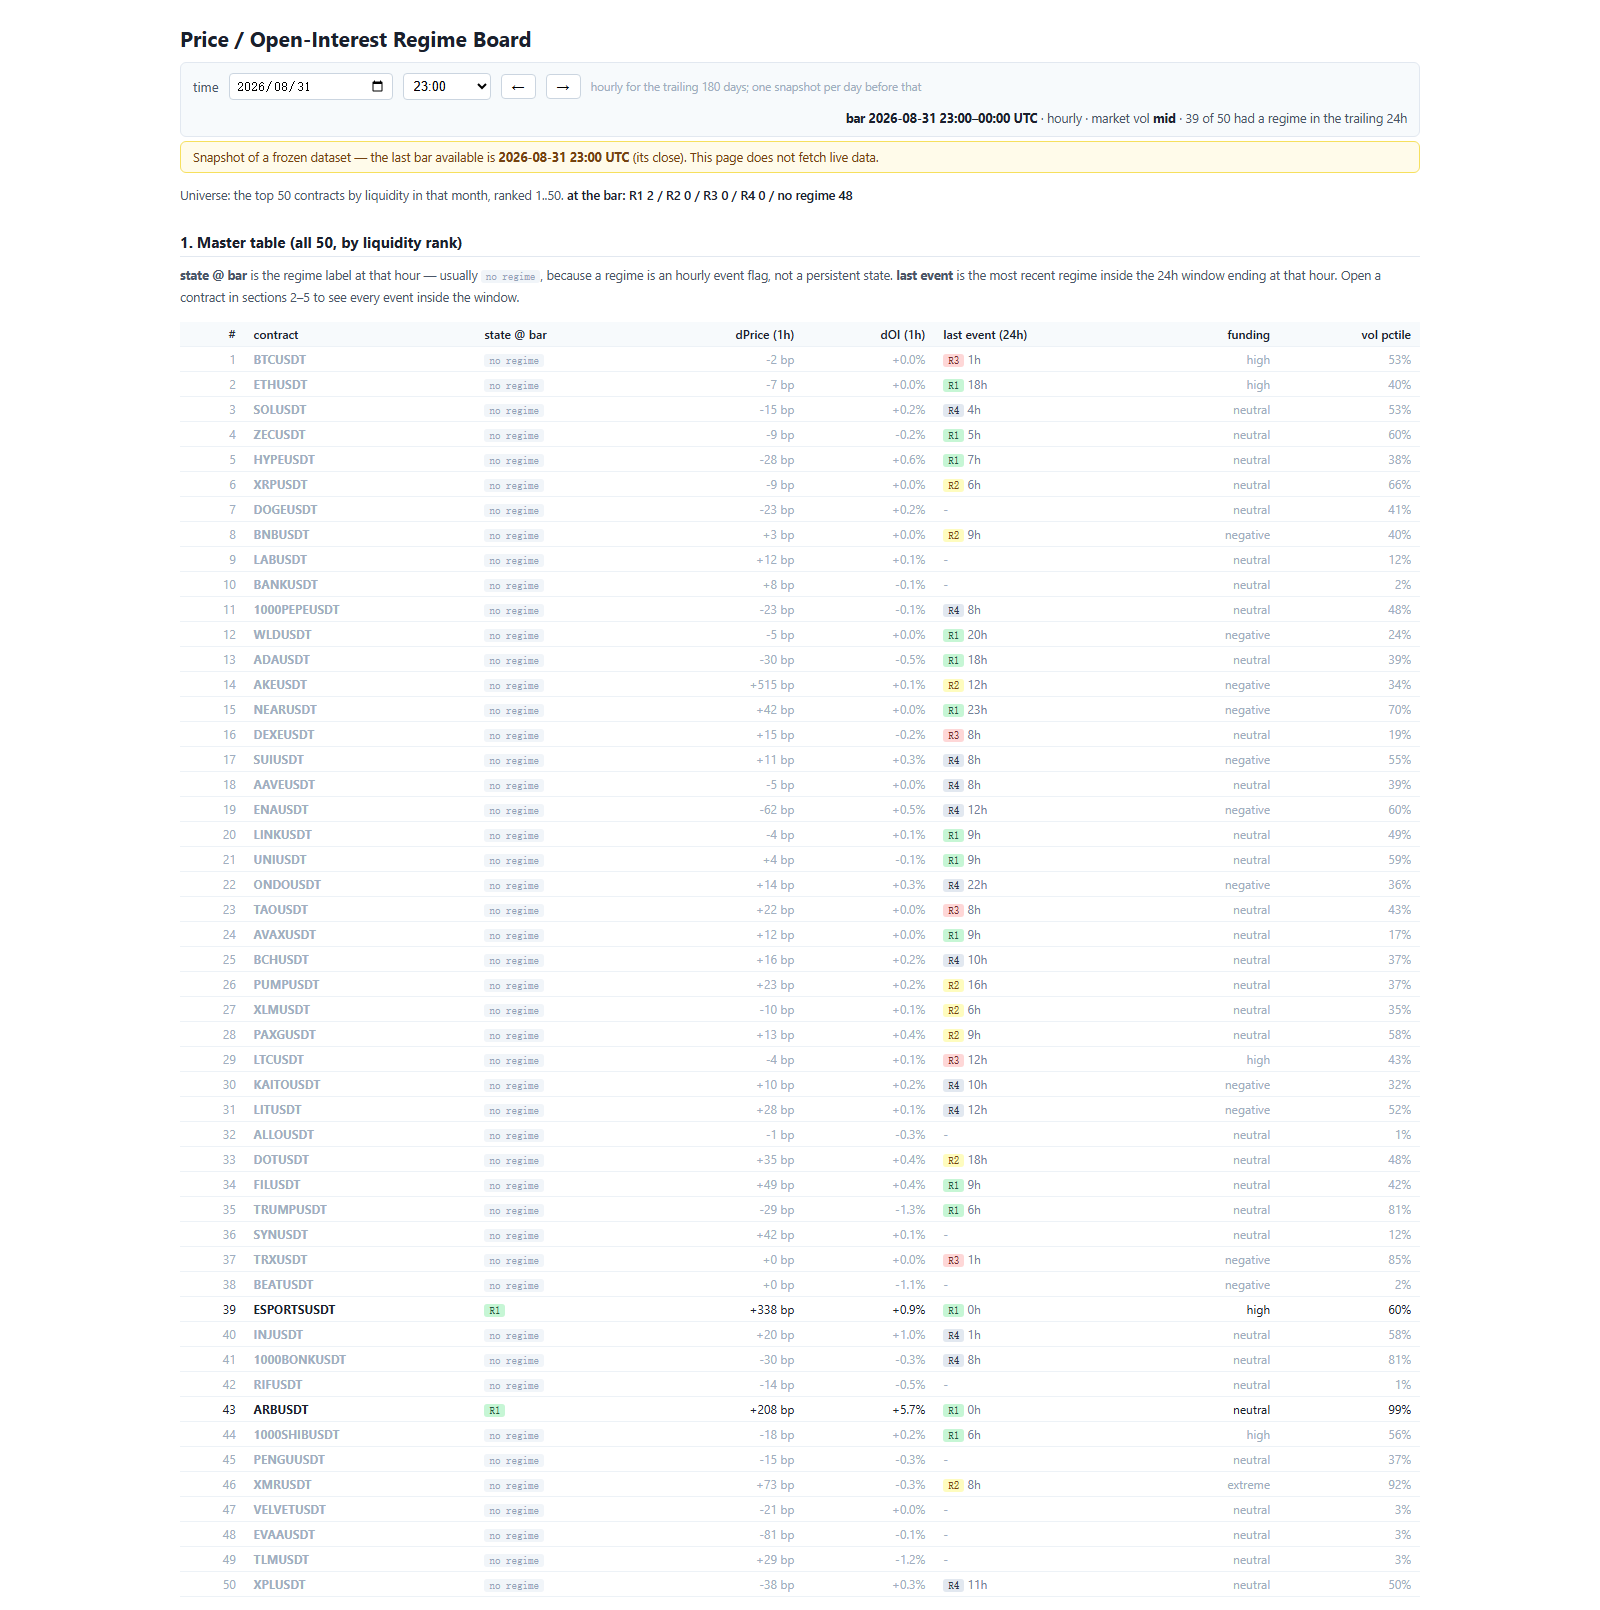
\includegraphics[width=0.92\linewidth,height=0.40\textheight,keepaspectratio]{figs/d5_master.png}
\caption{Master table, 2026-08-31 23:00 UTC. The state column is the regime label at the selected bar; the last-event column is the most recent regime inside the trailing 24 hours. At this hour 48 of the 50 contracts carry no label at the bar itself.}
\end{figure}

\begin{figure}[H]
\centering
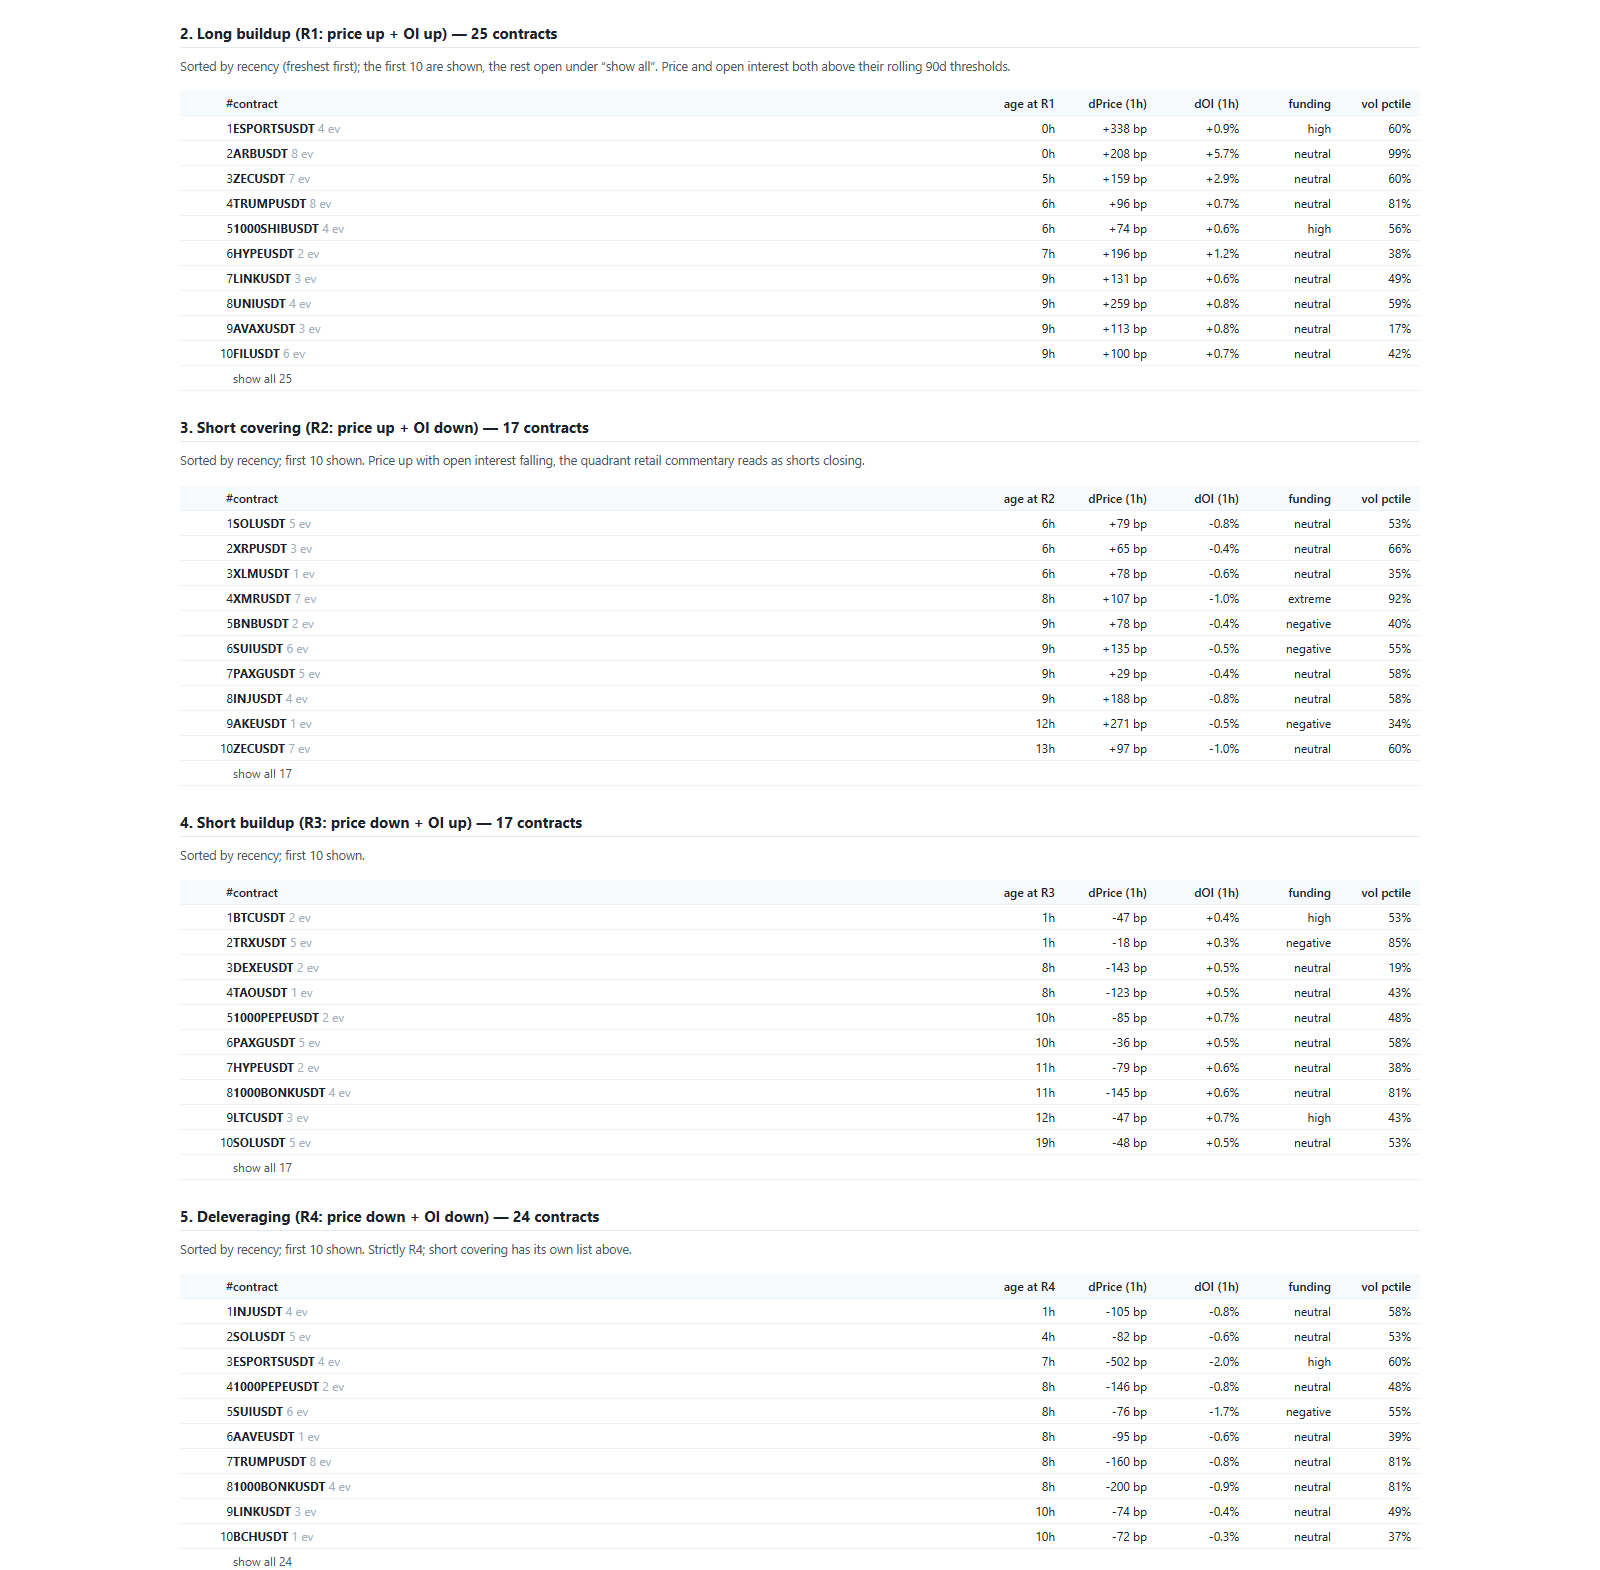
\includegraphics[width=0.92\linewidth,height=0.40\textheight,keepaspectratio]{figs/d5_events.png}
\caption{The four directional lists, 2026-08-31 23:00 UTC. Each list holds the contracts that had that quadrant inside the 24-hour window, ordered by the age of their latest event of that kind; a row expands to every event of any kind in the window.}
\end{figure}

\begin{figure}[H]
\centering
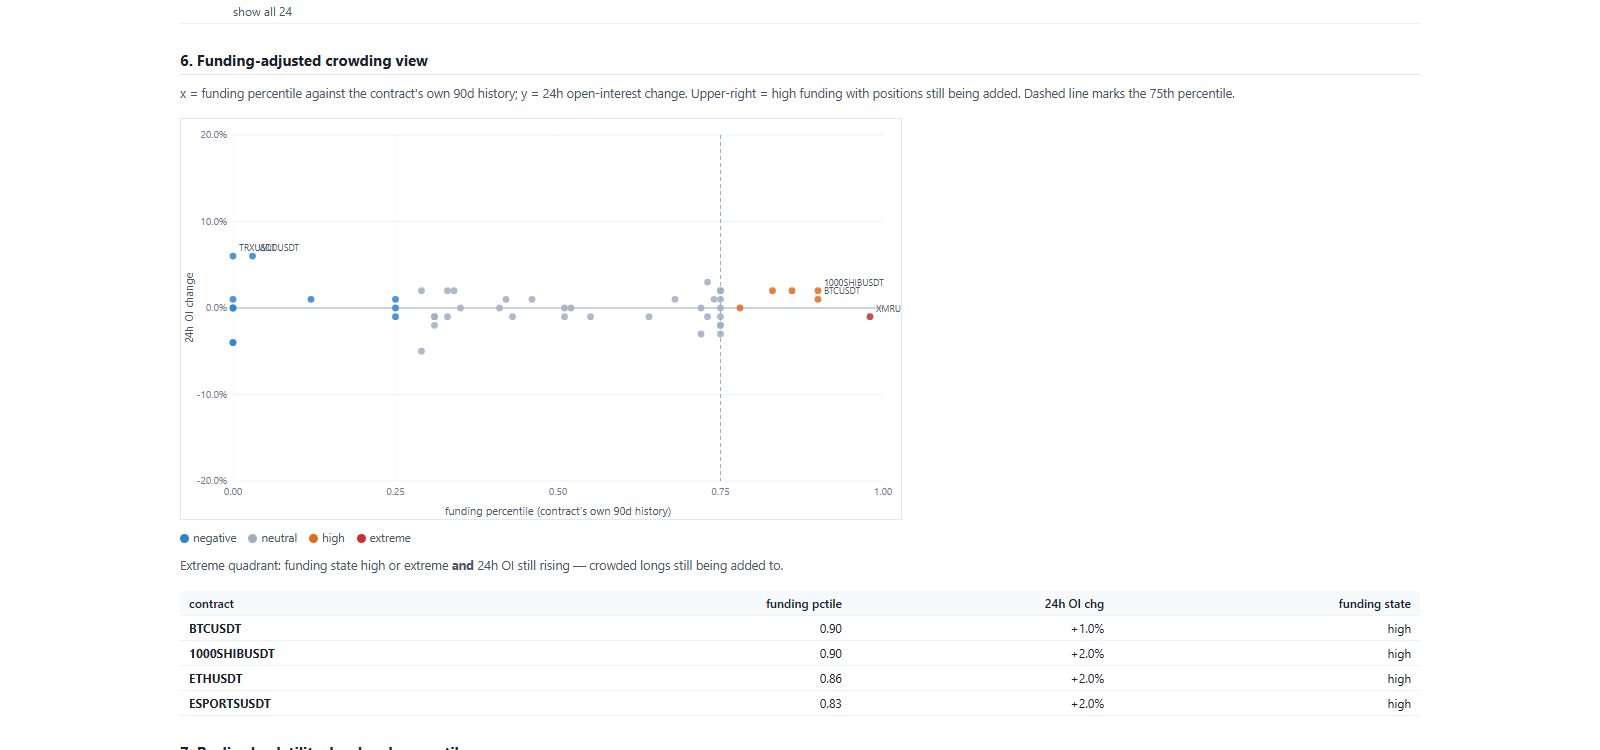
\includegraphics[width=0.92\linewidth,height=0.40\textheight,keepaspectratio]{figs/d5_crowding.png}
\caption{Funding-adjusted crowding, 2026-08-31 23:00 UTC. Funding percentile against the 24-hour change in open interest; the marked quadrant is high funding with positions still being added, and the table below lists the contracts inside it.}
\end{figure}

\begin{figure}[H]
\centering
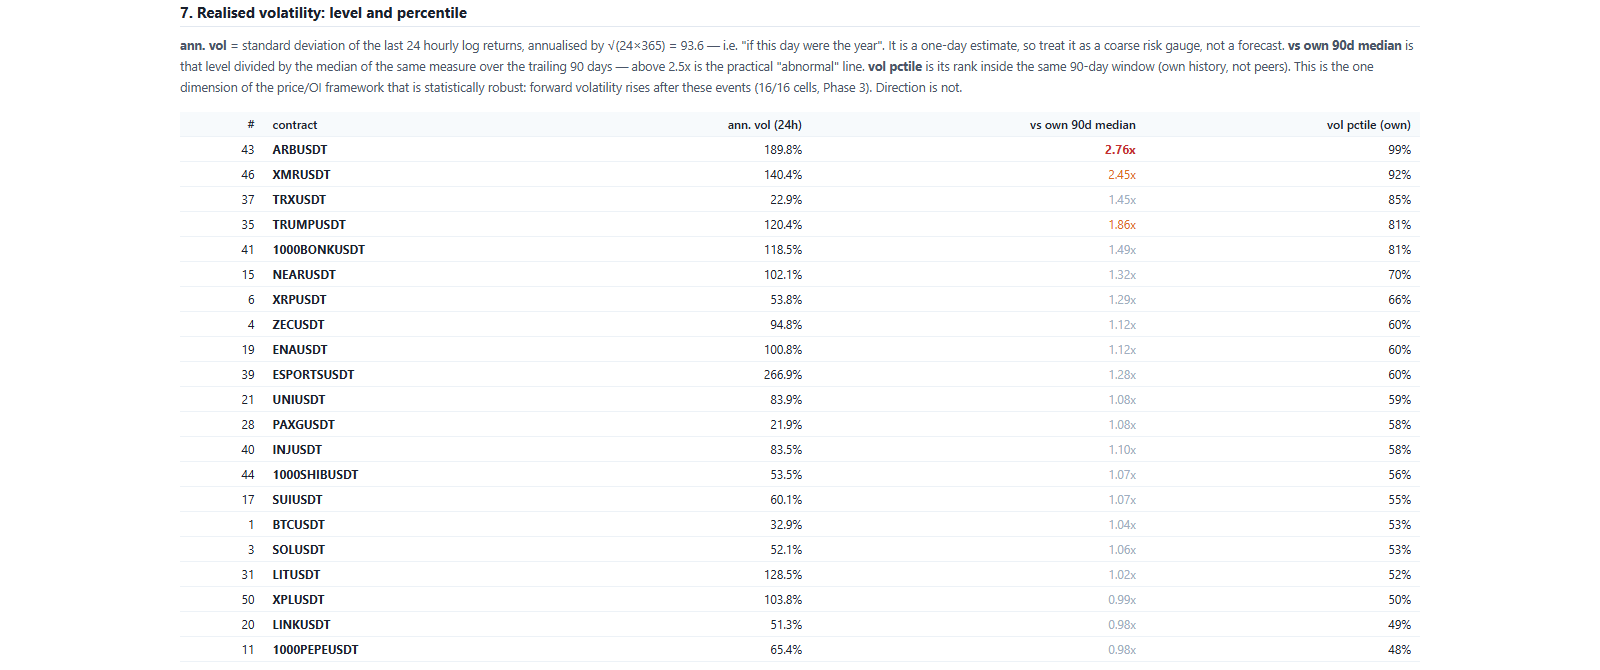
\includegraphics[width=0.92\linewidth,height=0.40\textheight,keepaspectratio]{figs/d5_vol.png}
\caption{Realised volatility, 2026-08-31 23:00 UTC. Annualised 24-hour realised volatility, the ratio to its own rolling 90-day median, and the percentile within the contract's own history; ratios above 2.5x are shaded.}
\end{figure}

\bigskip

\section{Results and Findings}

\subsection{Phase 3: what a regime carries}

Volatility is the one result that survives every check. Each cell is compared with the other rows that crossed the same price threshold in the same direction but do not belong to that cell, so the benchmark is the rest of the price move. All 16 cell-horizon estimators are positive, survive BH correction and survive dropping the five most influential contracts, and Figure 7 shows every one of them above its benchmark. The gain is largest at short horizons and shrinks as the window lengthens.

\begin{figure}[H]
\centering
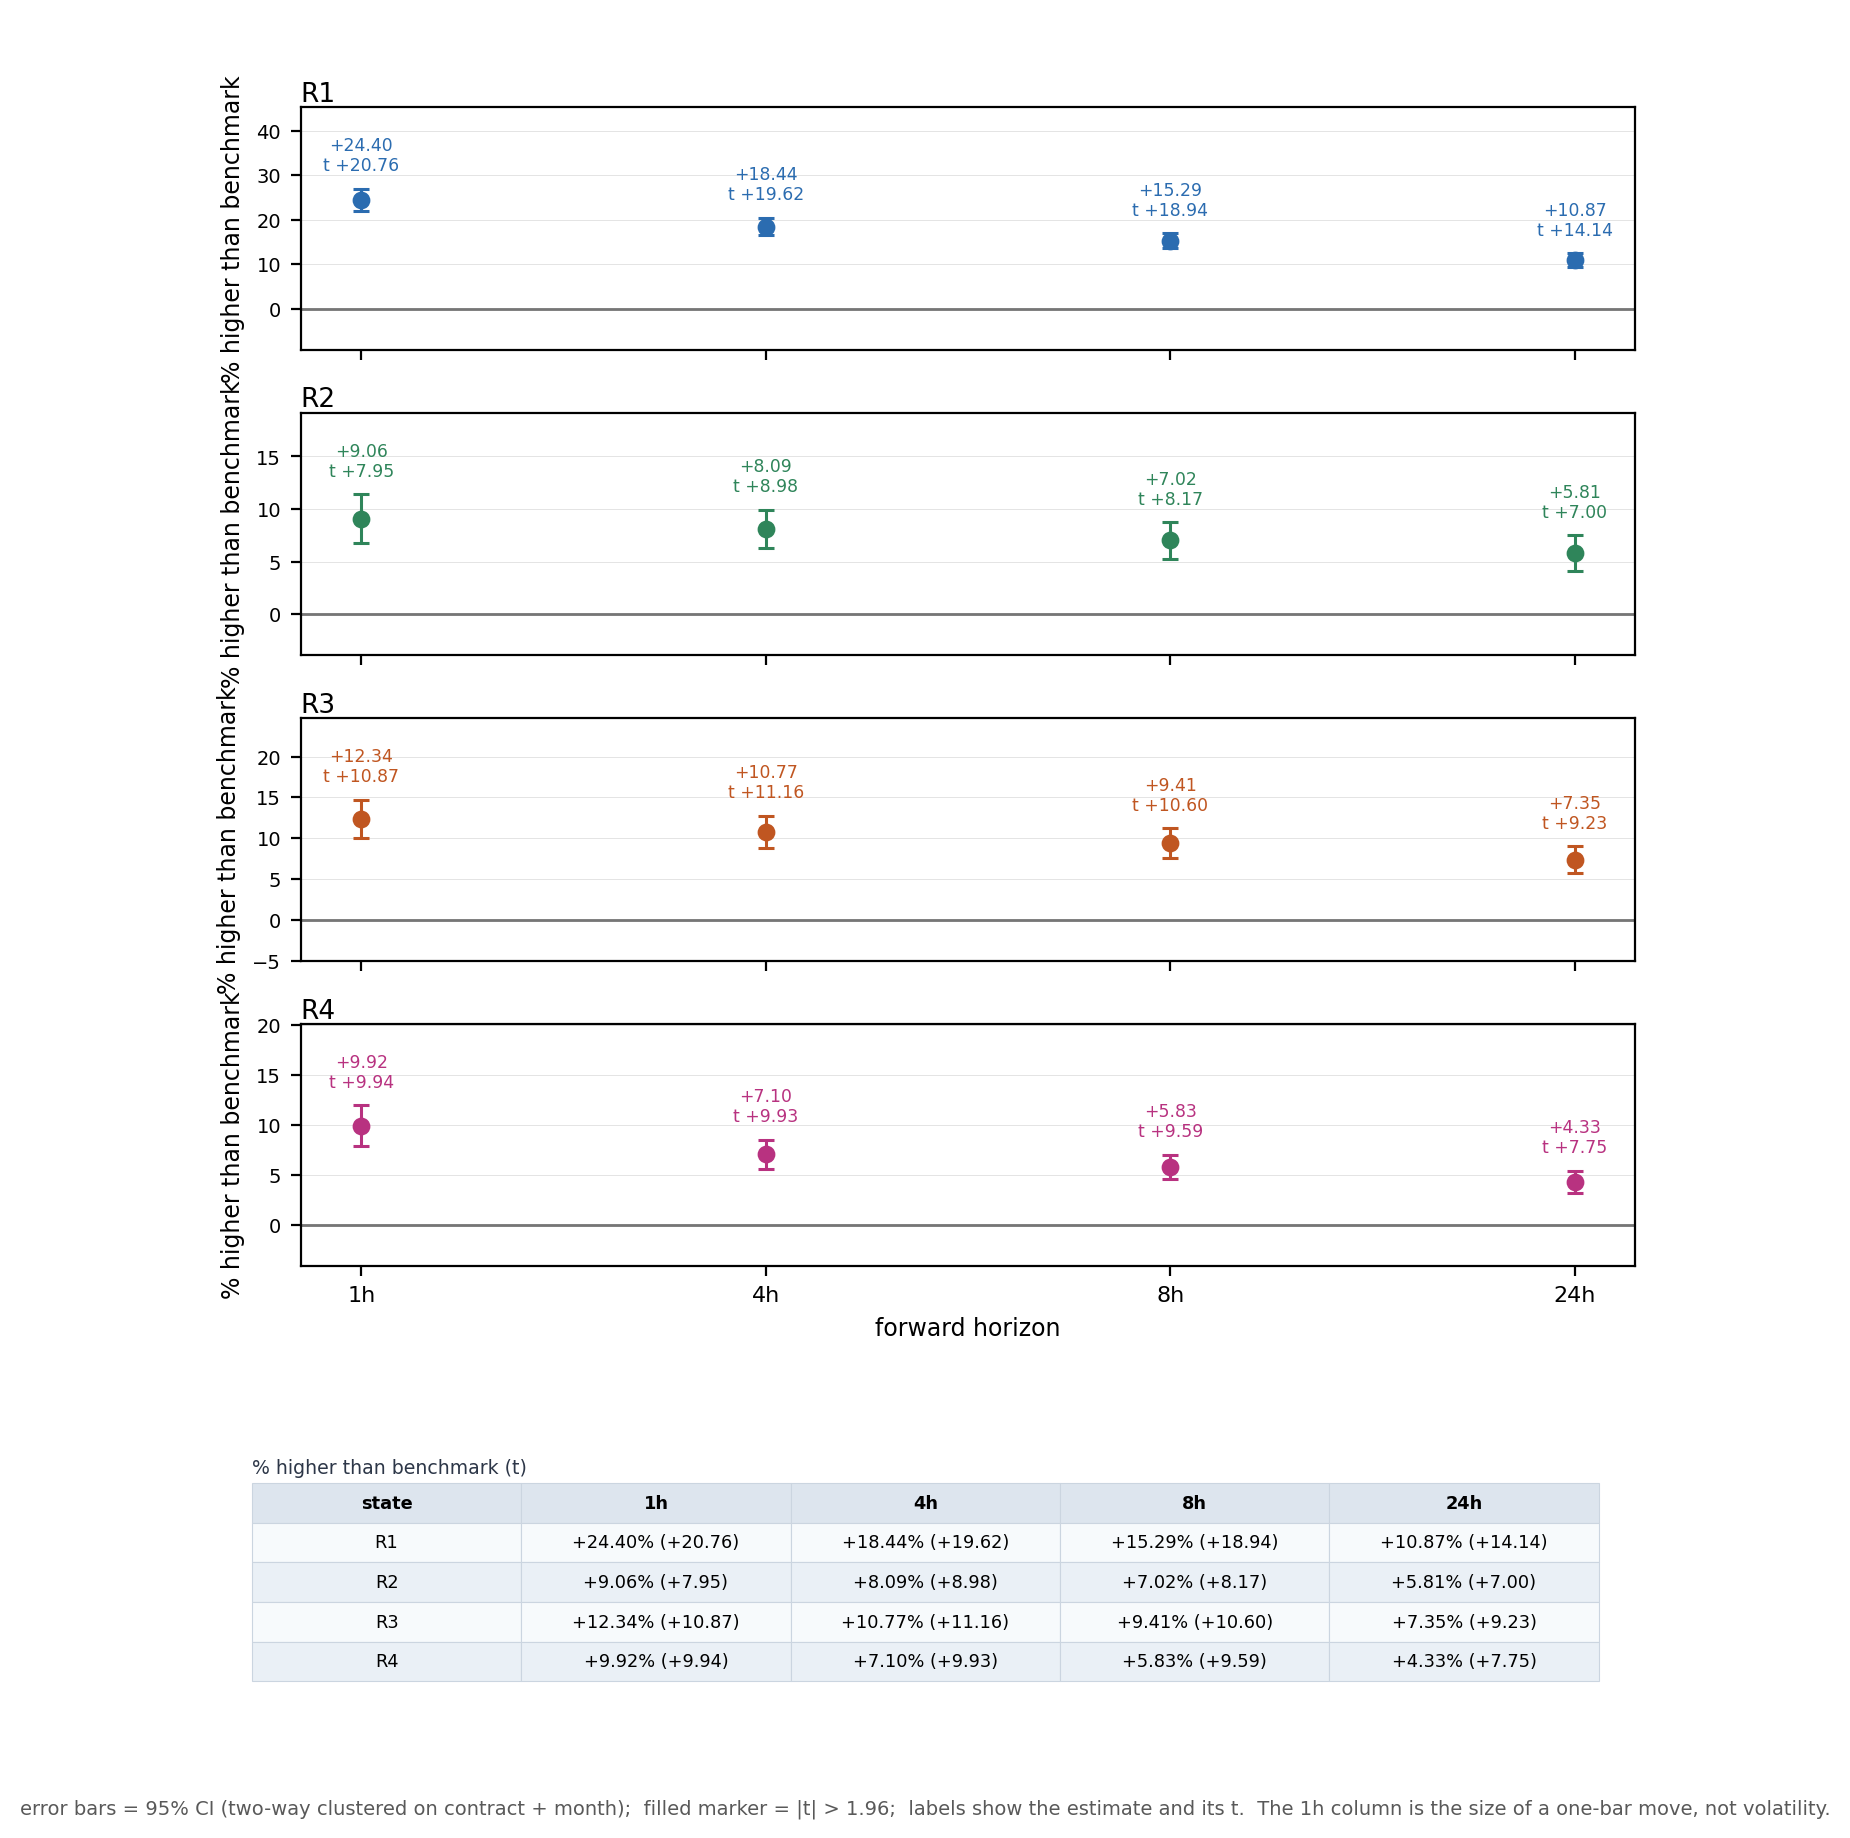
\includegraphics[width=0.92\linewidth,height=0.40\textheight,keepaspectratio]{figs/r1_volatility.png}
\caption{Forward realised volatility by cell and horizon, as a percentage of the price-matched benchmark. Bars are 95\% intervals; filled markers are |t| > 1.96.}
\end{figure}

Figure 8 repeats the layout for direction, and most intervals cross zero. 6 of the 16 increments are significant, two positive and four negative. The larger positive is +2.51 bp, for R1 at one hour; the larger negative is $-$11.63 bp, for R3 at twenty-four hours. Both are small, and the signs are not consistent across cells.

\begin{figure}[H]
\centering
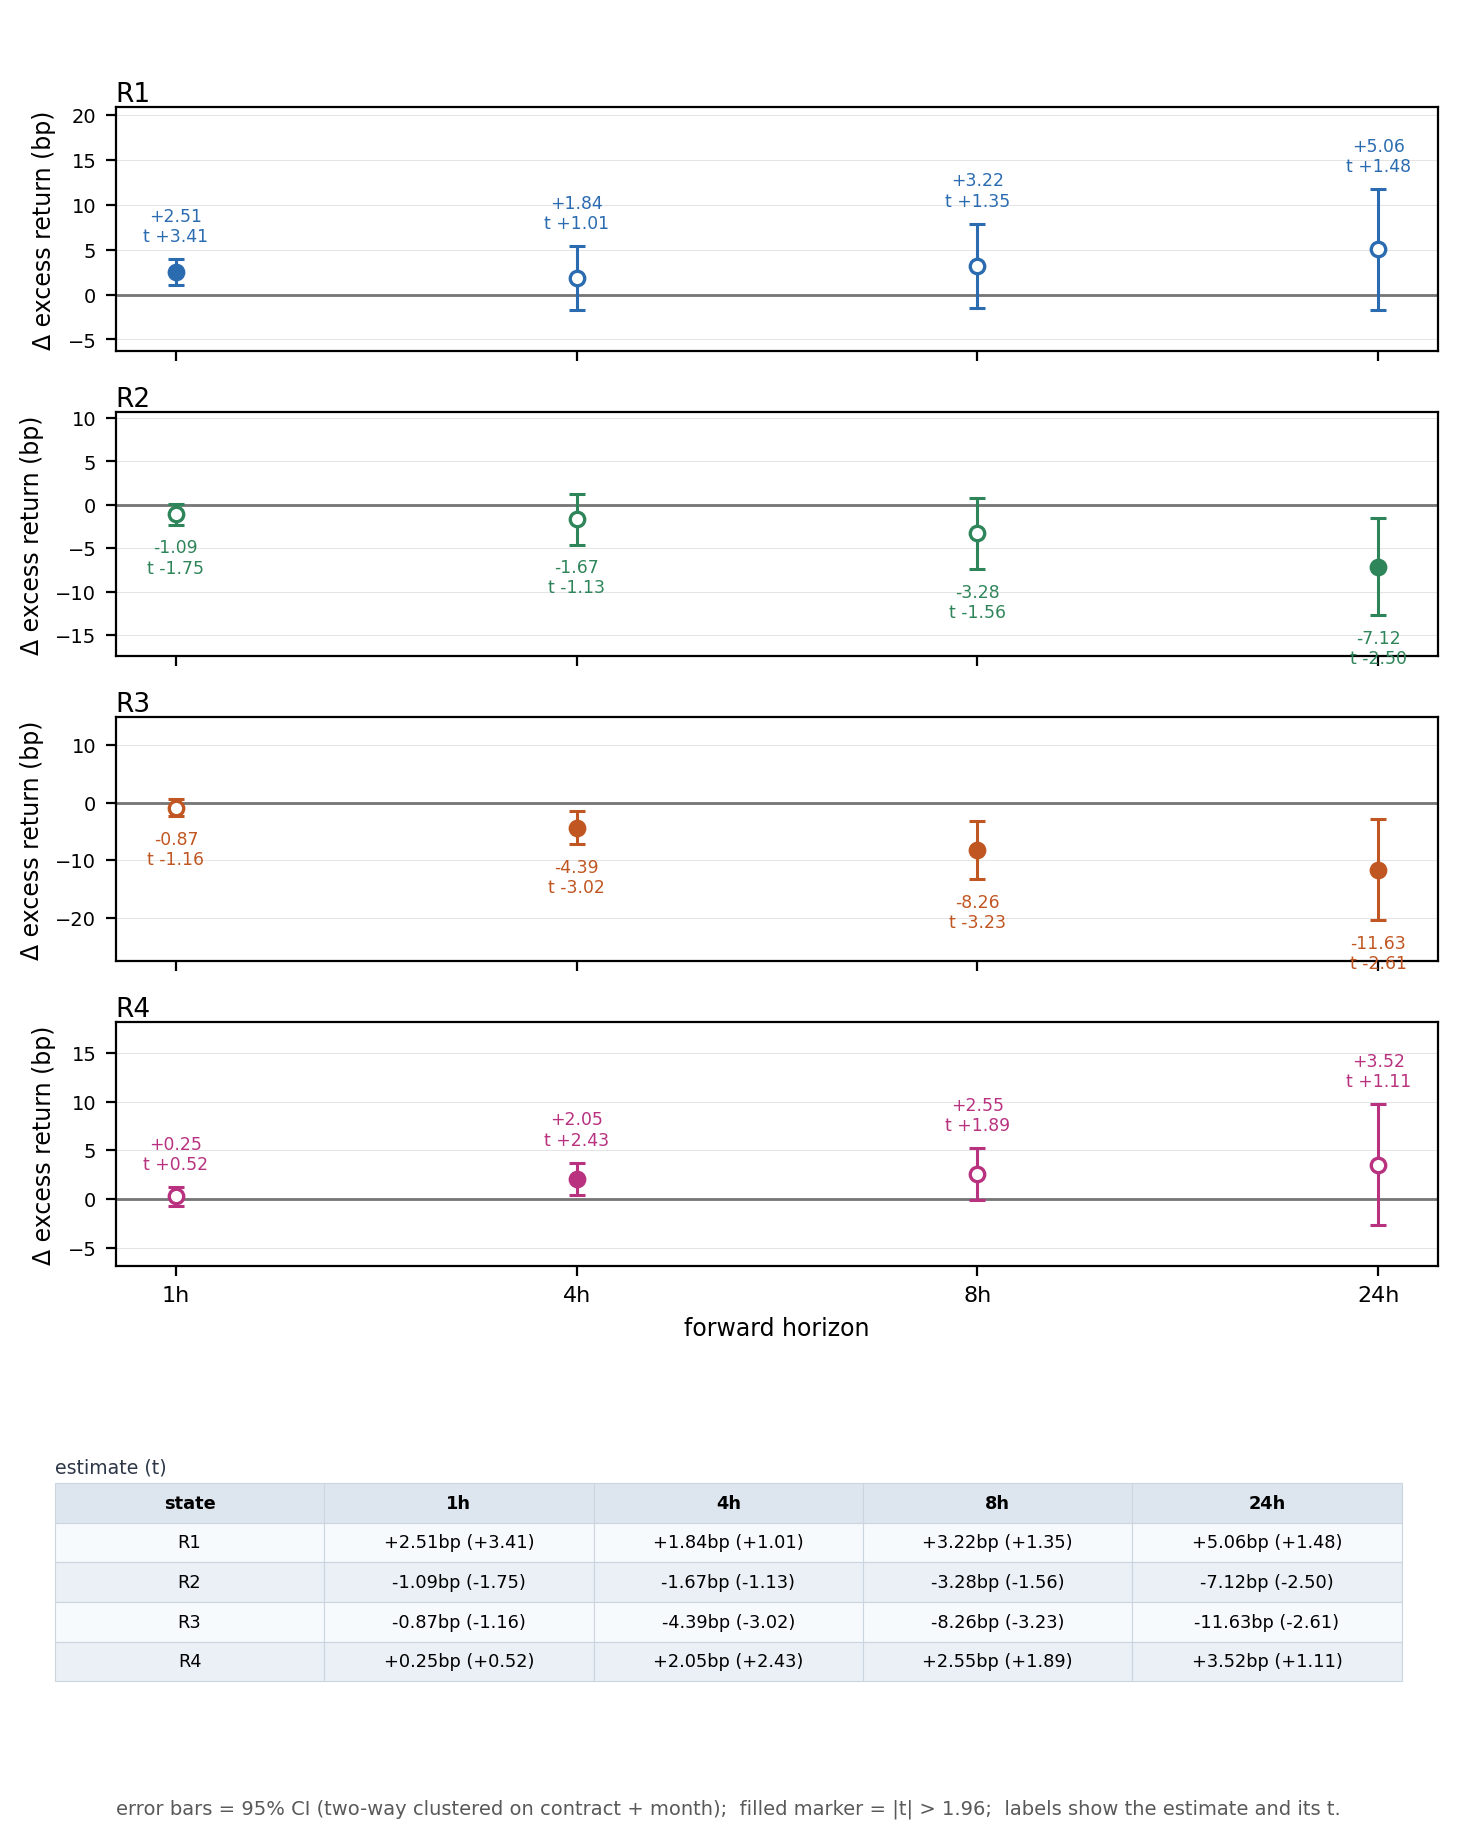
\includegraphics[width=0.92\linewidth,height=0.40\textheight,keepaspectratio]{figs/r1_direction.png}
\caption{Mean forward return by cell and horizon, as a difference from the same-direction benchmark, in basis points. Error bars are 95\% intervals from two-way clustering; filled markers are |t| > 1.96.}
\end{figure}

The direction result depends on how hours are counted. Under event weighting every event-hour is one; under contract-day weighting the hours inside a contract-day are averaged first, so a day with many events counts once and within-day variation drops out. Figure 9 shows that the contrast flips sign in all four cells. The top row shows why the unit matters: a day's mean return depends on how many hours the state appeared, rising for R1 from $-$20.6 bp at one hour to +33.5 bp at five or more and falling for R3 from +6.3 to $-$30.6.

\begin{figure}[H]
\centering
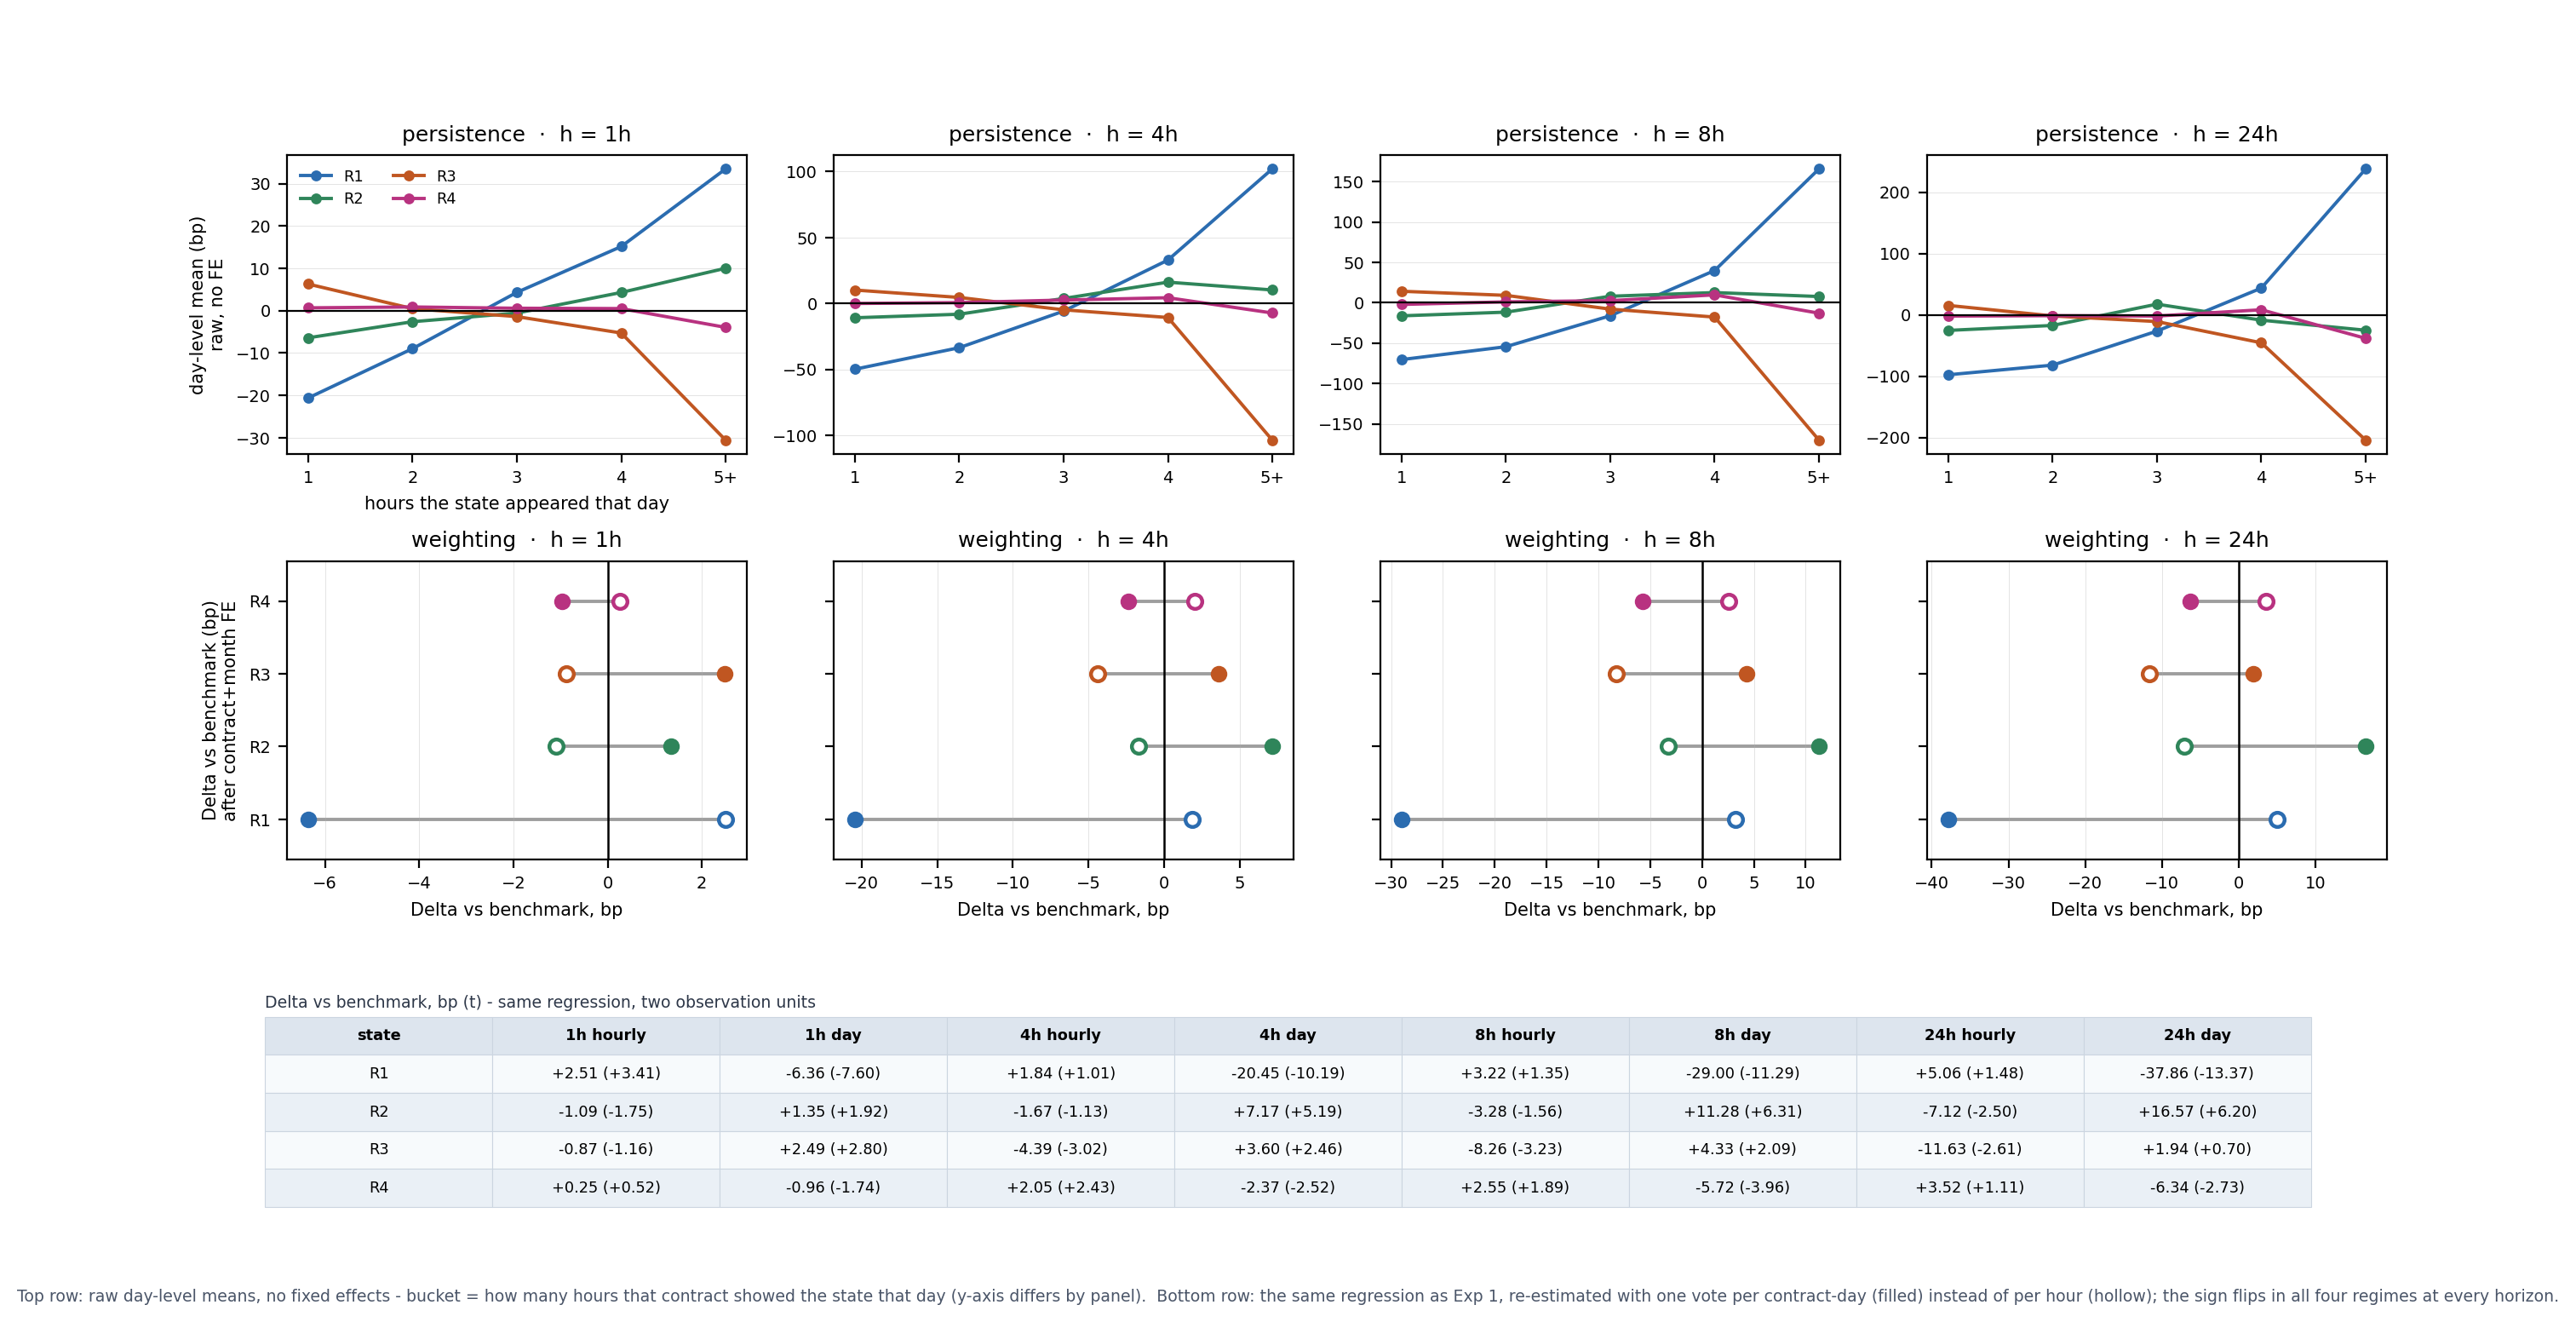
\includegraphics[width=0.92\linewidth,height=0.40\textheight,keepaspectratio]{figs/r1_weighting.png}
\caption{The return result by weighting and by within-day persistence. Top: day-level mean return against the number of hours the state appeared that day, raw and without fixed effects; the y-axis differs by panel. Bottom: the same regression as Figure 8, with one vote per contract-day (filled) instead of per hour (hollow); the table gives every estimate with its t.}
\end{figure}

A significant increment is not a level a trader can hold. Table 1 gives the market-neutral level of every cell at every horizon.

\begin{table}[H]\centering
\caption{Table 1. Forward return by cell and horizon, market-neutral, in basis points.}
\footnotesize
\begin{tabularx}{\linewidth}{>{\raggedright\arraybackslash}X>{\raggedleft\arraybackslash}X>{\raggedleft\arraybackslash}X>{\raggedleft\arraybackslash}X>{\raggedleft\arraybackslash}X}
\toprule
Cell & 1h & 4h & 8h & 24h \\
\midrule
R1 & +0.70 & $-$0.84 & $-$1.15 & $-$3.26 \\
R2 & $-$2.30 & $-$3.90 & $-$6.67 & $-$13.70 \\
R3 & $-$0.57 & $-$5.91 & $-$11.31 & $-$20.51 \\
R4 & +0.22 & +0.42 & $-$0.08 & $-$4.76 \\
\bottomrule
\end{tabularx}
\end{table}

\emph{Market-neutral means of the forward return.}

Every cell is negative at twenty-four hours, from $-$3.26 bp for R1 to $-$20.51 bp for R3, and every one is lower there than at one hour. Beating a benchmark that also loses money leaves the level negative, which is why the gate tests the level rather than the increment.

The two effects are not additive. The price-by-open-interest interaction is positive at every horizon, +3.46, +6.81, +12.22 and +20.67 bp, with t-statistics from 2.8 to 4.3: what a change in open interest does depends on which way price moved, which is what the four-quadrant reading asserts and what a two-signal rule would miss.

\begin{figure}[H]
\centering
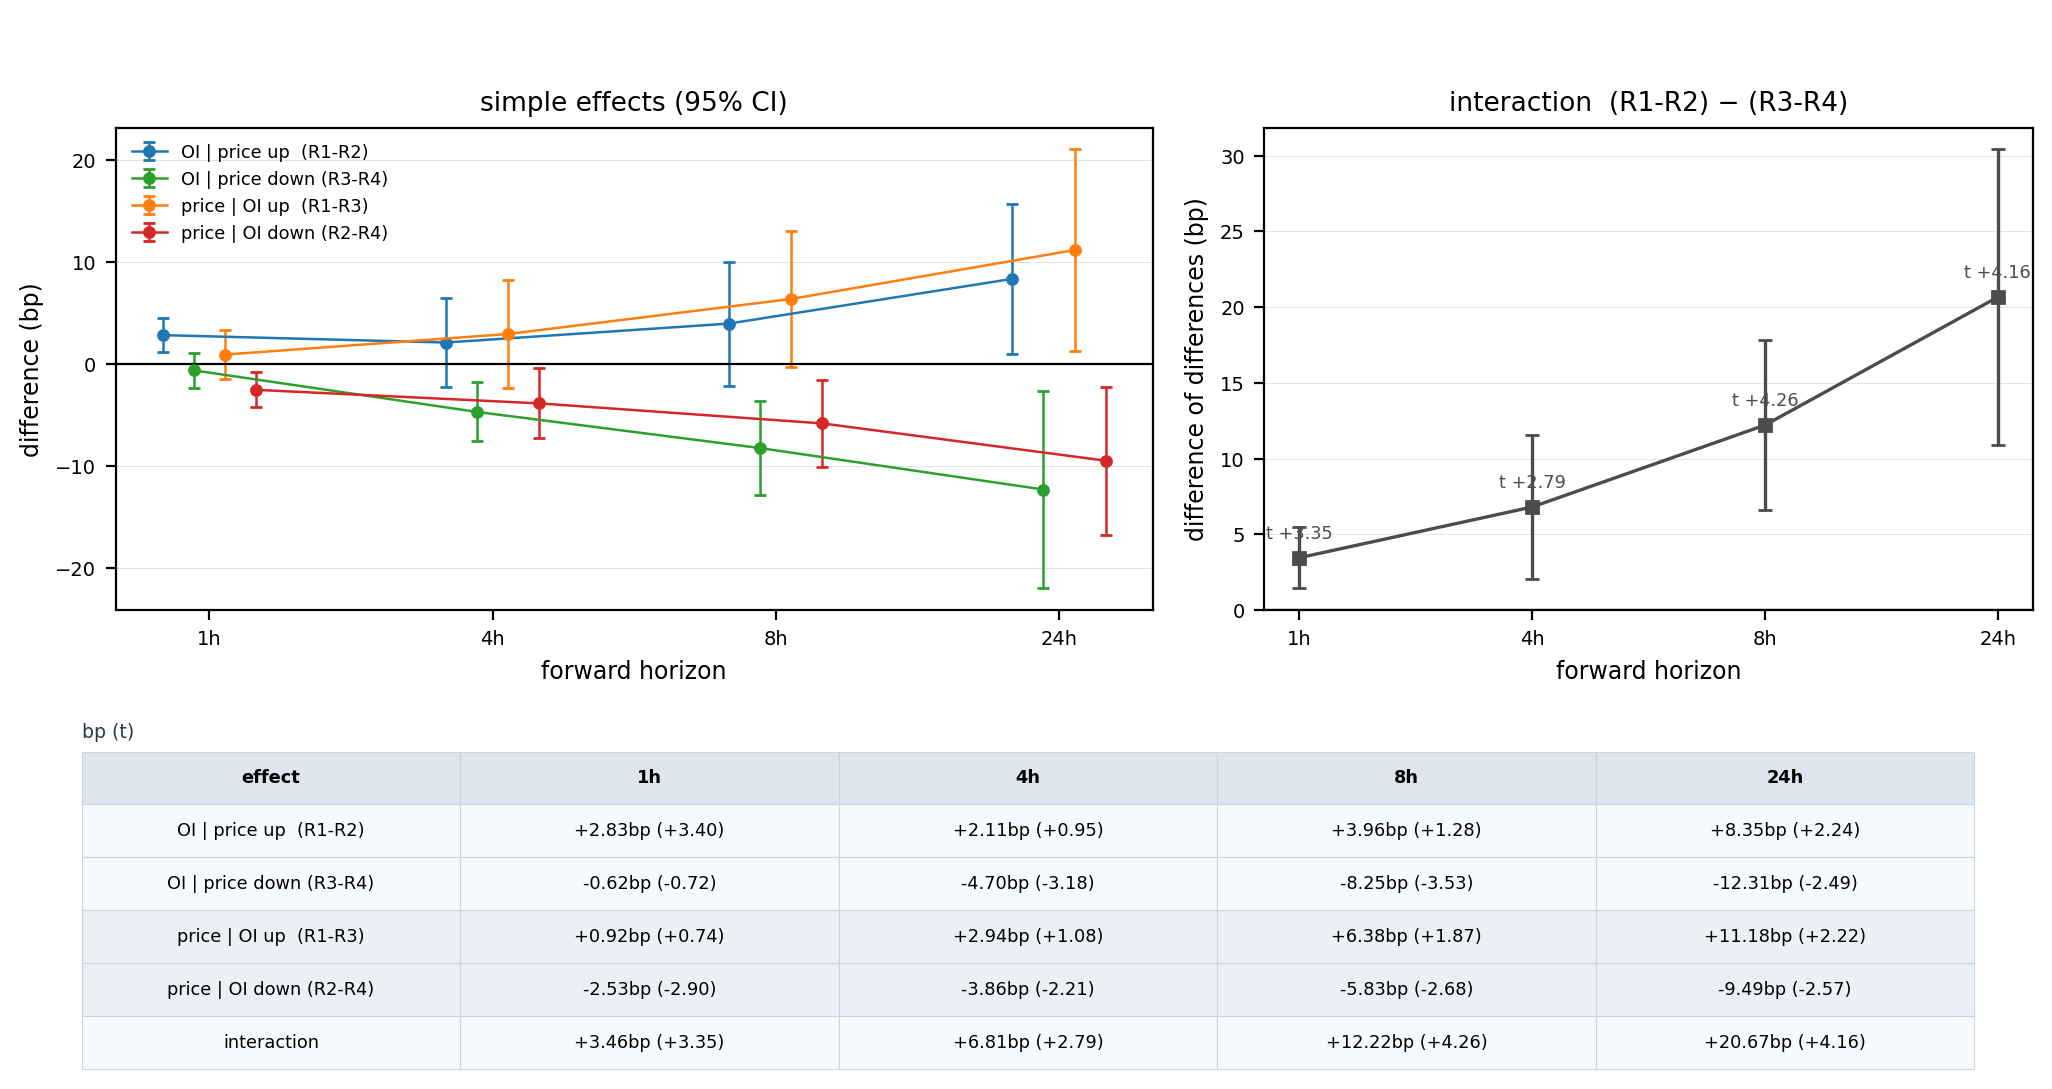
\includegraphics[width=0.92\linewidth,height=0.40\textheight,keepaspectratio]{figs/r1_interaction.png}
\caption{The price-by-open-interest interaction. Left: simple effects, each the difference between two cells along one dimension. Right: the interaction, (R1 $-$ R2) $-$ (R3 $-$ R4), which rises with the horizon; t in labels, bars are 95\% intervals. The table gives every effect with its t.}
\end{figure}

Reversal is more frequent than continuation in every cell, 50--54\% against 45--50\%; at twenty-four hours, R1 is 2.5 pp more likely to reverse than its benchmark and R2 1.9 pp less. The majority outcome is still the losing one, so the minority continuation must carry the larger payoff.

\begin{figure}[H]
\centering
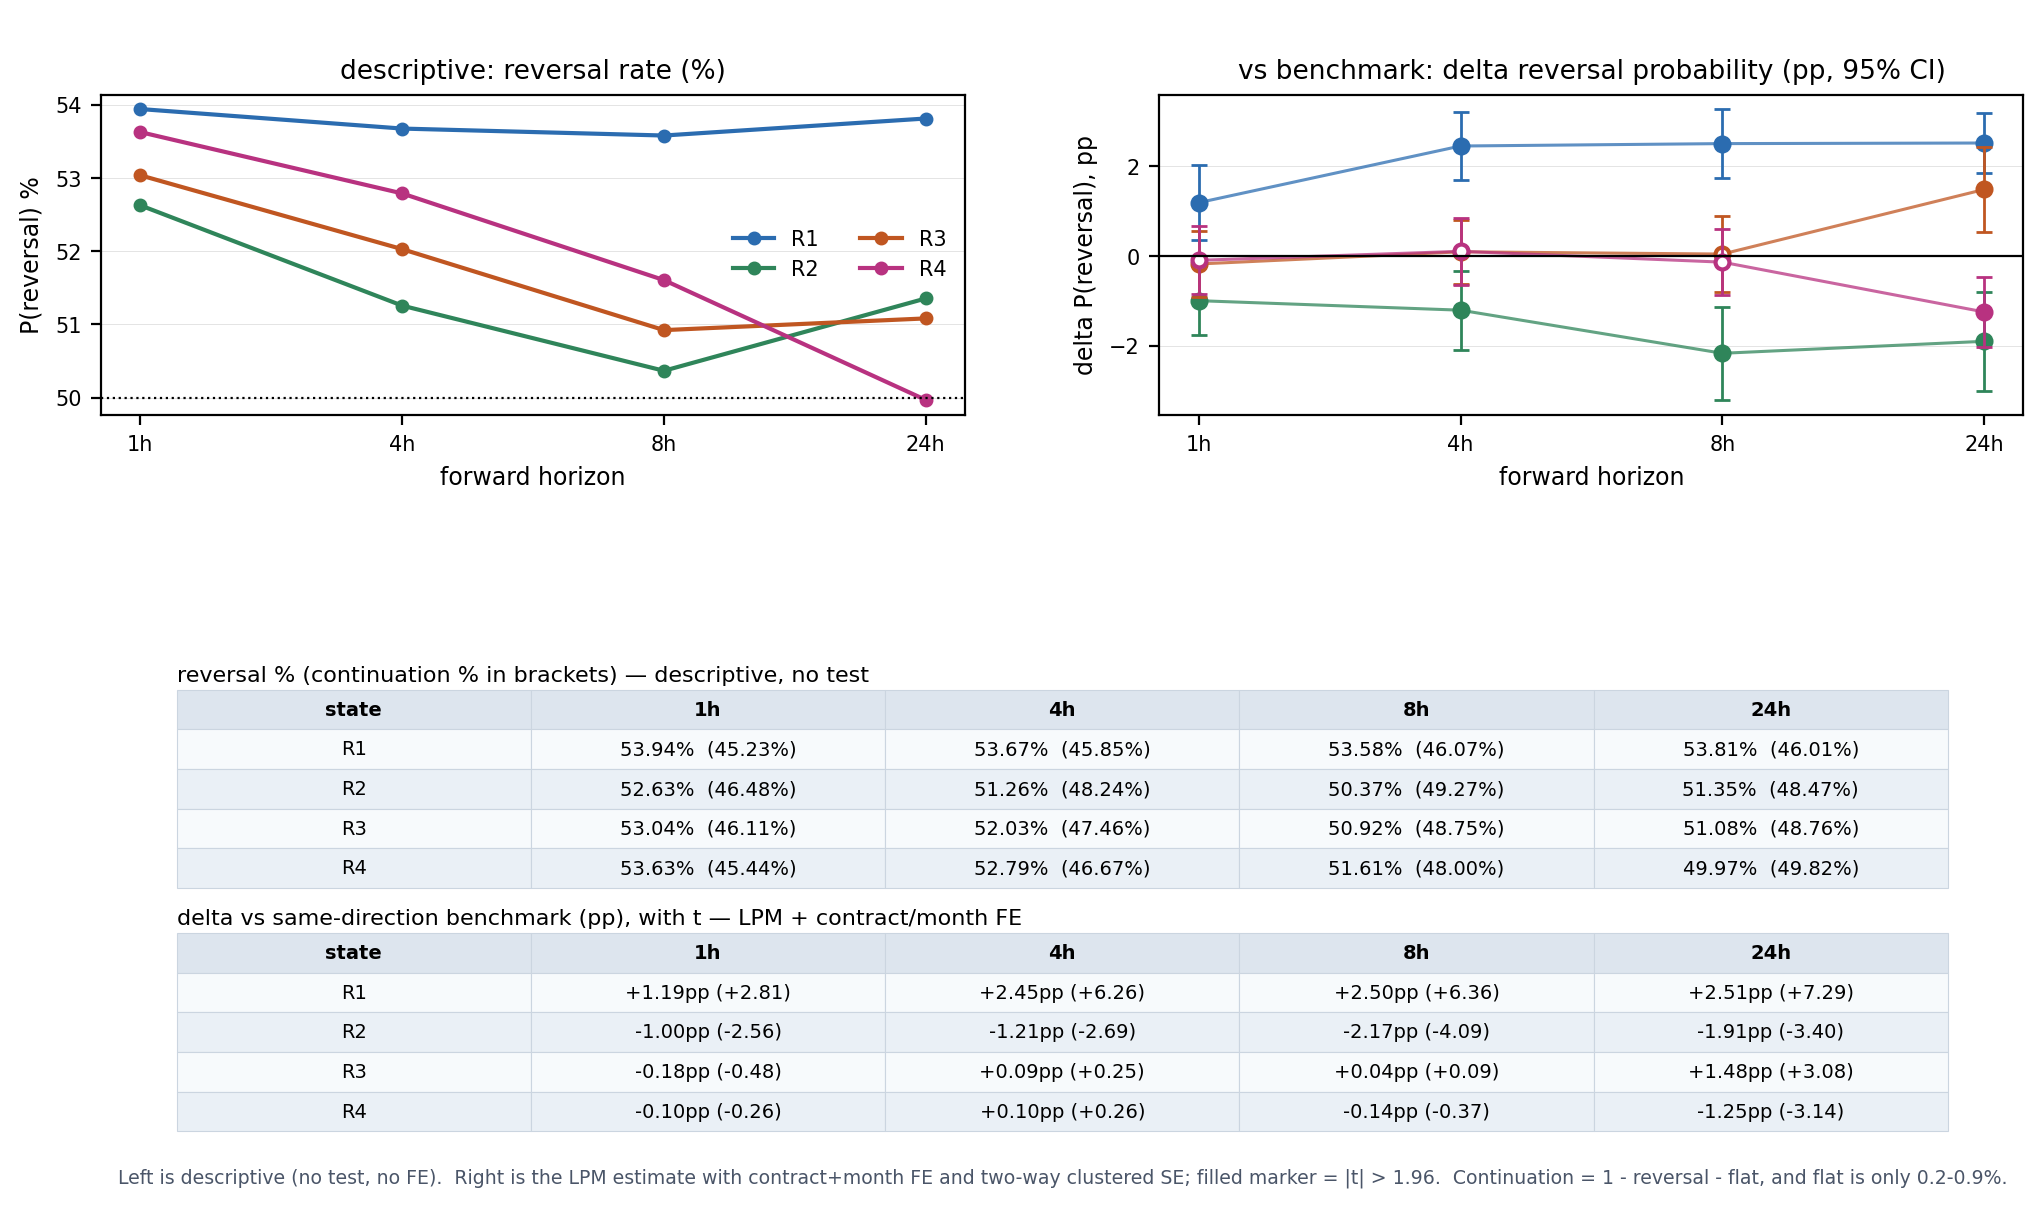
\includegraphics[width=0.92\linewidth,height=0.40\textheight,keepaspectratio]{figs/r1_reversal.png}
\caption{Reversal behaviour. Left: the raw reversal rate, descriptive. Right: the gap to the same-direction benchmark from a linear probability model with contract and month effects; filled markers are |t| > 1.96.}
\end{figure}

\subsection{The framework against single-signal baselines}

In this section, single-signal baselines are discussed. Price only goes long when price crosses its threshold upward and short when it crosses downward; open interest only applies that rule to the change in open interest and ignores price; funding only goes long when funding sits in its top two states and short when it is negative. Random timing draws the same contracts and the same number of events at random hours.

The four-state rule itself is long R1 and short R4. Nobody would hold that as a real trading position: the two legs are picked for symmetry rather than for trading. The rule keeps the four-state spread on the same footing as the single-signal rules, so that it can be compared with each baseline.

None of the three baselines is profitable after costs. Their pooled long-short spreads run from $-$6.42 bp for funding alone at twenty-four hours to +0.63 bp for open interest alone at one hour, and none survives Benjamini--Hochberg correction at any horizon. Against that floor the four-state rule gains nothing: of twelve day-level differences with the three baselines, only one passes |t| > 1.96 and none survives the BH correction.

\begin{figure}[H]
\centering
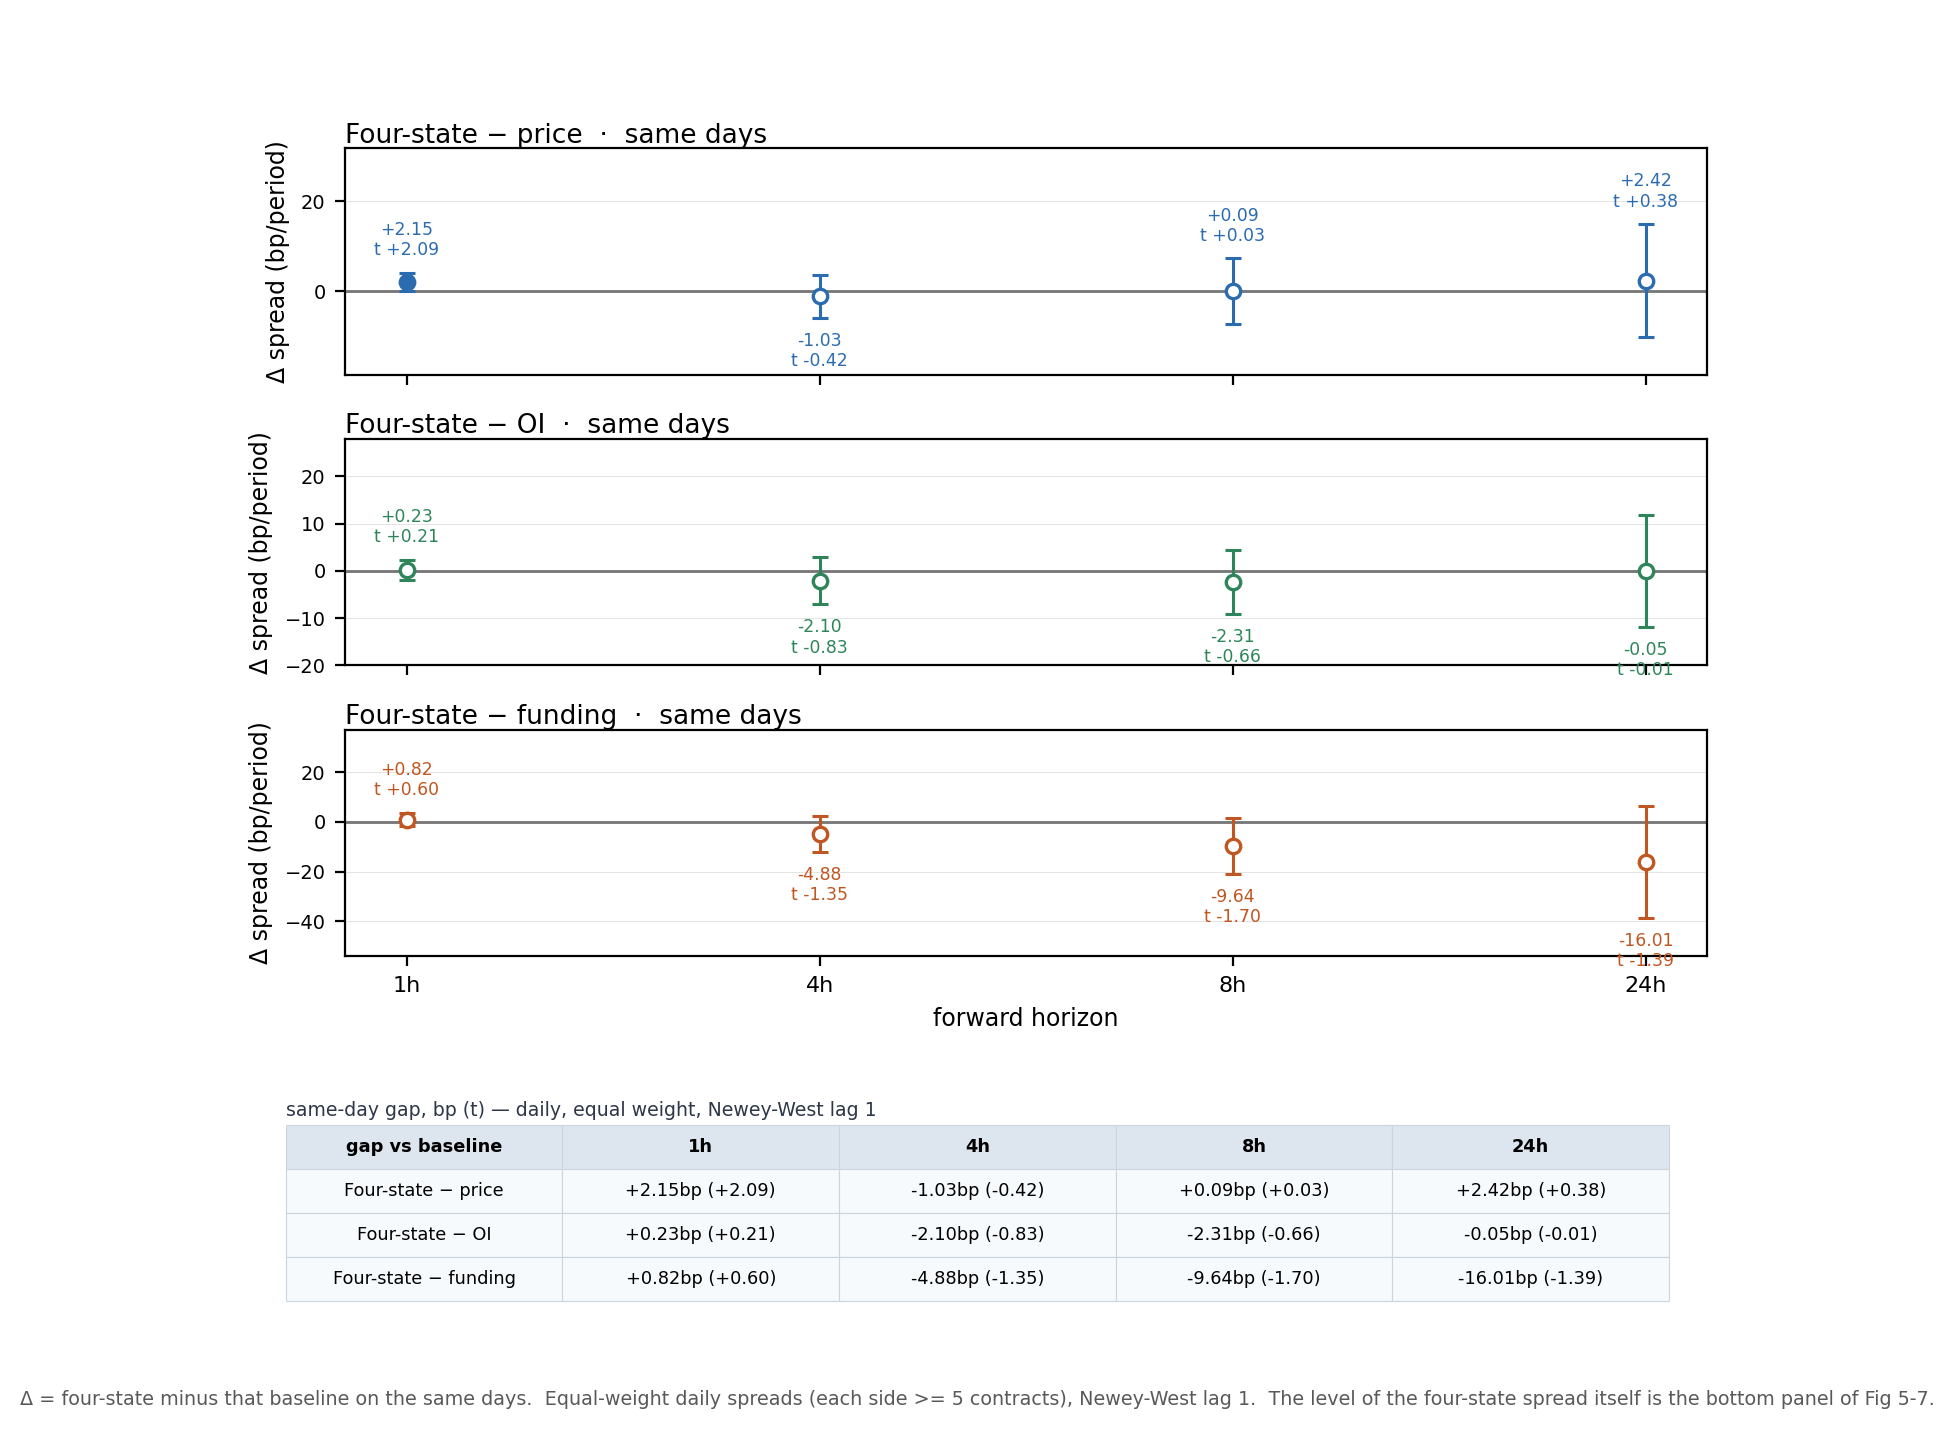
\includegraphics[width=0.92\linewidth,height=0.40\textheight,keepaspectratio]{figs/r2_baselines.png}
\caption{The four-state spread minus each single-signal baseline on the same days, in basis points, with the underlying gaps in the table. Delta is the four-state rule minus that baseline; error bars are 95\% intervals from a Newey-West lag-1 estimator.}
\end{figure}

The timing is not arbitrary. Against 1,000 random draws of the same contracts with the same number of events each, ten of sixteen cells fall outside the 5--95\% band. Seven fall below it and three above, so the states select hours that differ from random timing, and mostly differ for the worse. The framework can select, but it cannot profit.

\begin{figure}[H]
\centering
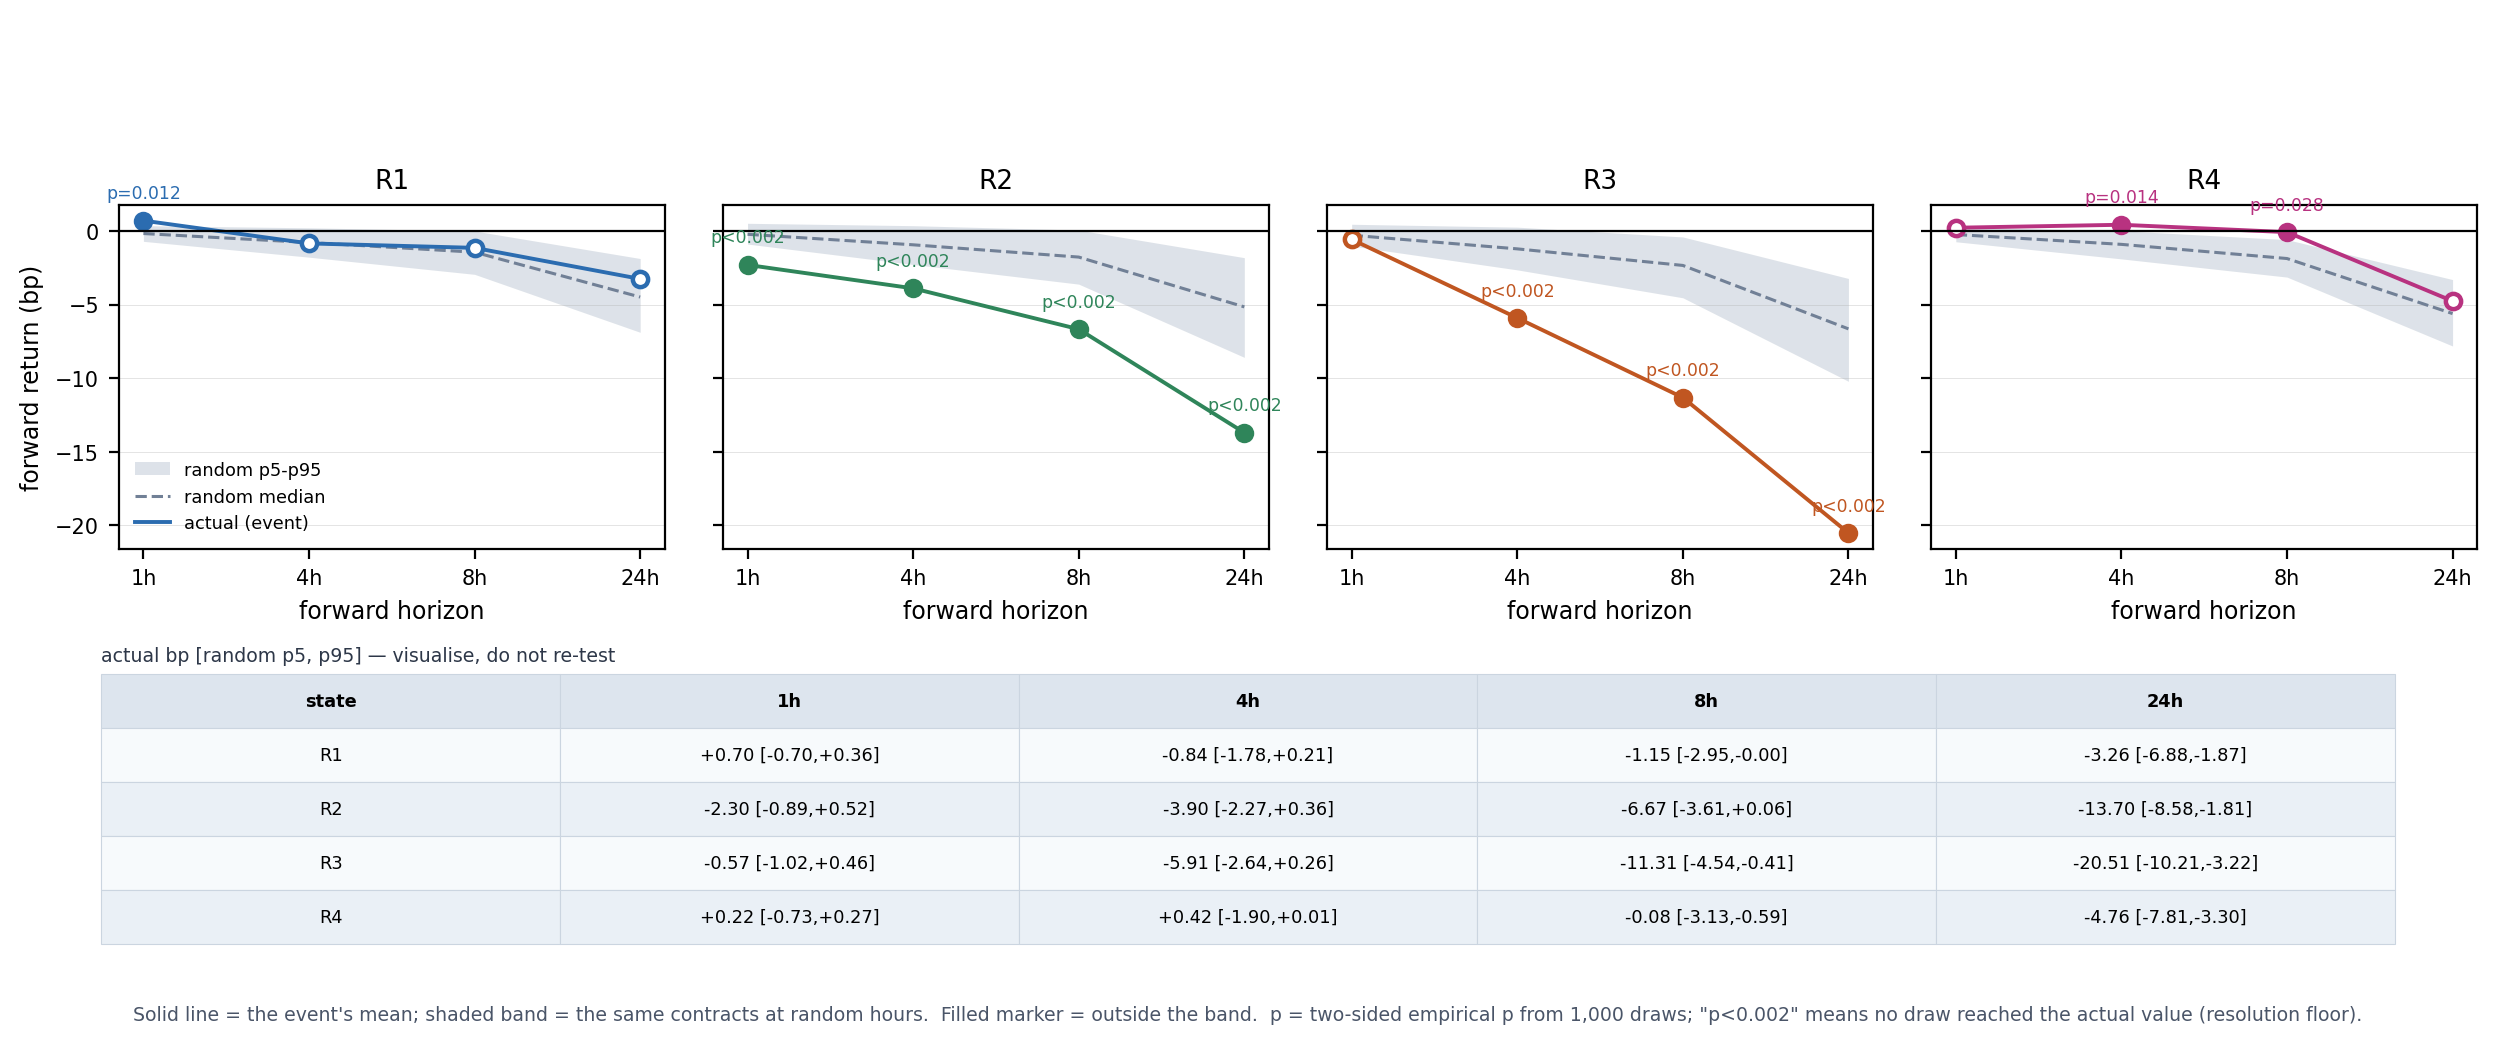
\includegraphics[width=0.92\linewidth,height=0.40\textheight,keepaspectratio]{figs/r2_placebo.png}
\caption{Event return against the same contracts at random hours. The shaded band is the 5--95\% range of 1,000 draws per contract, the dashed line the median draw; filled markers fall outside the band, and the table gives the actual value with its confidence interval.}
\end{figure}

\subsection{Phase 4: does funding change anything}

Funding conditions the size of the next move, not its direction. Forward volatility is higher in every funding state than at neutral, continuation and reversal shift only when funding is negative, and the mean return barely moves at all.

\begin{itemize}
\item Volatility responds at almost every horizon. Eighty-three of the ninety-six log-volatility contrasts survive BH correction and the drop-5 check, and all are positive: +6.1\% on average for negative funding against neutral, +10.1\% for high and +17.6\% for extreme. Distance from neutral matters, not its sign, so both tails carry more volatility than the middle. The thirteen failures sit in the negative column, seven of them in R1, and four at R3 high and extreme at one hour.
\end{itemize}

\begin{itemize}
\item Reversal shifts only in the negative tail, and splits by direction. Seven contrasts survive, all of them negative against neutral. Where price rose, negative funding makes continuation more likely: $-$1.84 pp for R1 at one hour and $-$2.46 for R2 at eight. Where price fell, the same state makes reversal more likely: +1.46 pp for R4 at one hour, +2.86 for R3 at eight and +2.64 at twenty-four.
\end{itemize}

\begin{itemize}
\item The mean return barely moves. Two of ninety-six contrasts survive, both at one hour under contract-day weighting: R4 at +2.47 bp and R3 at +5.29 bp. Their levels are +2.04 and +5.56 bp, so even if the contrast is real, a long position earns under six basis points before a 20 bp round trip.
\end{itemize}

Figure 14 lays out all ninety-six contrasts, one column per outcome and one row per horizon; the three bullets follow its columns.

\begin{figure}[H]
\centering
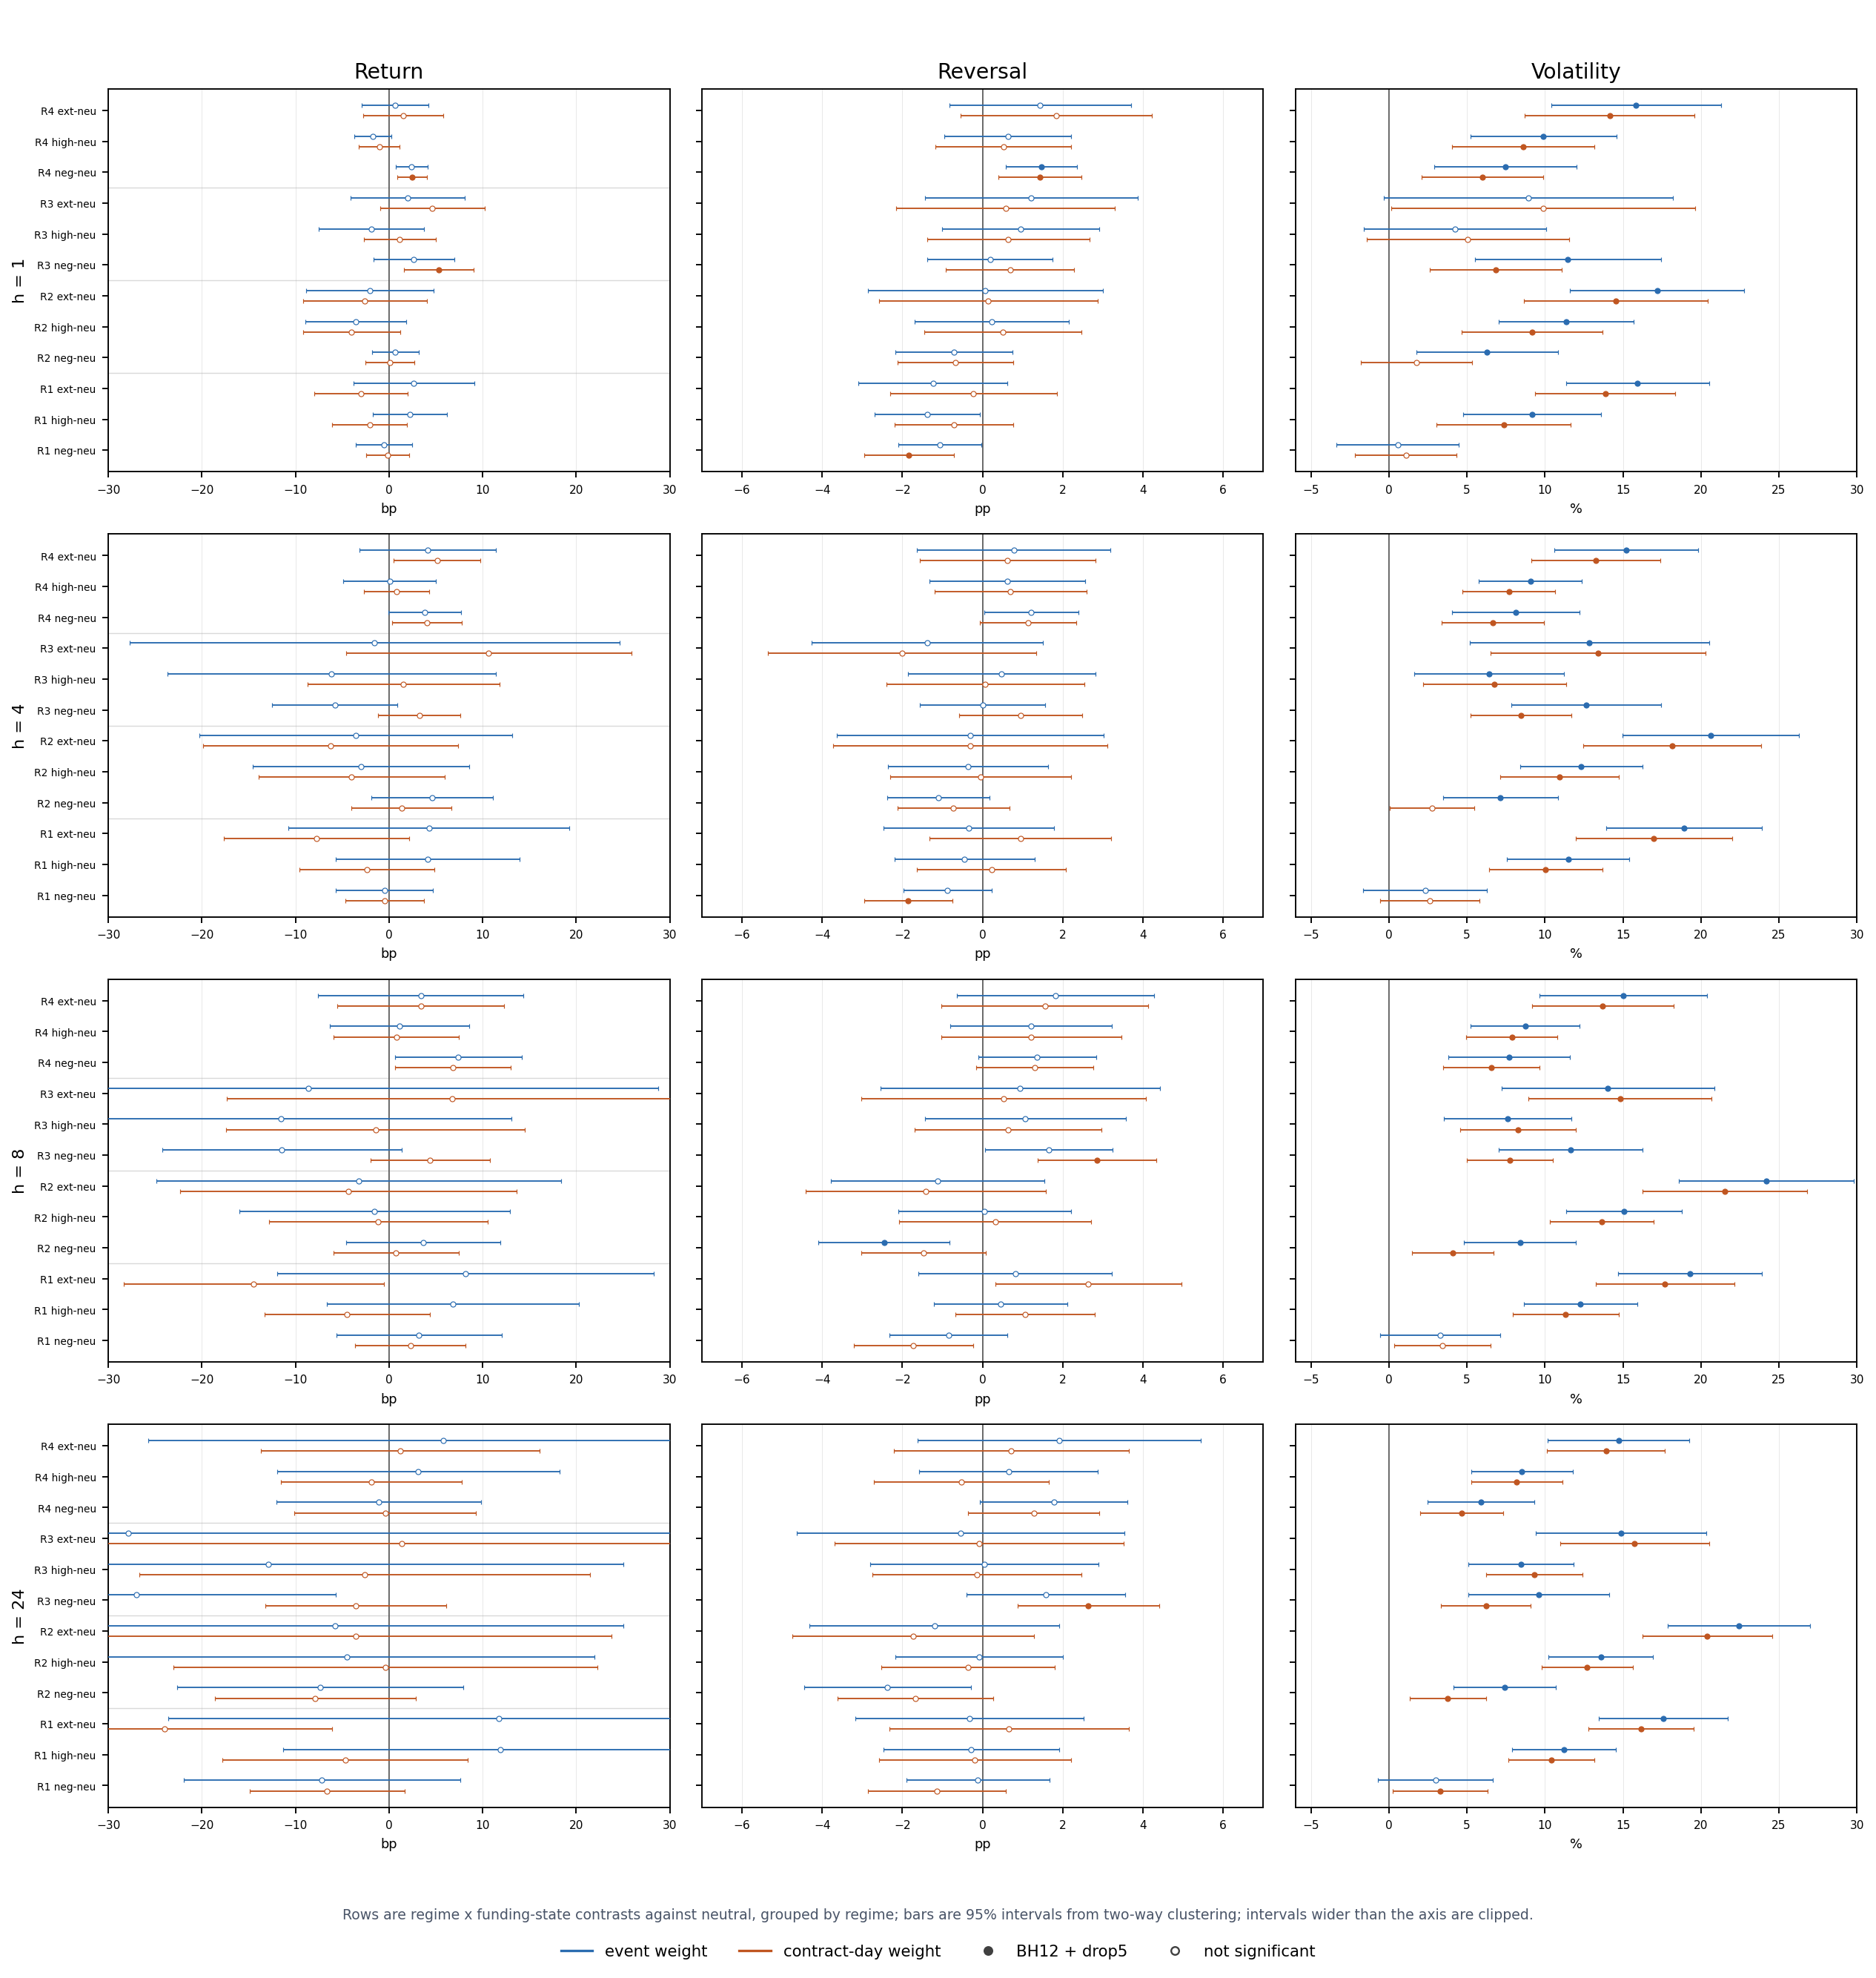
\includegraphics[width=0.92\linewidth,height=0.40\textheight,keepaspectratio]{figs/r2_panorama.png}
\caption{Within-regime funding contrasts at every horizon. Columns are the three outcomes, rows the four horizons; each row inside a panel is one regime crossed with one funding state against neutral. Blue is event-weighted, brown contract-day-weighted, filled markers survive BH and drop5 within a family of twelve, and intervals wider than the axis are clipped.}
\end{figure}

\subsection{Phase 5: can it be traded}

The ninety-six candidates are four regimes crossed with six conditioning states, three of funding and three of market volatility, at four horizons each. The two sets do not overlap: a candidate is conditioned on funding or on volatility, never on both. Funding enters the gate as negative, neutral and high; high covers both the high-only and the extreme-only rows, because the extreme-only cells are too thin to carry a test of their own.

\begin{table}[H]\centering
\footnotesize
\begin{tabularx}{\linewidth}{>{\raggedright\arraybackslash}X>{\raggedright\arraybackslash}X}
\toprule
Stage & Surviving candidates \\
\midrule
Candidate cells & 96 \\
G1: level different from zero, two-sided, BH-controlled & 10 (7 long, 3 short) \\
G2: market-neutral mean on the trade's side & 7 (4 long, 3 short) \\
G3: median and trimmed mean, 1\% from each tail, on the trade's side & 4 (all long) \\
G4: stability across years and trailing 12 months & 2 (all long) \\
G5: mapped to executable strategies & 2 (A1, B1) \\
\bottomrule
\end{tabularx}
\end{table}

Each gate rules out a different way for a backtest to lie. G1 asks whether the forward return is distinguishable from zero at all, two-sided, with the sign of the estimate setting the side. G2 asks whether it survives removing the market mean return, since a cell that only rises with the market is beta rather than signal. G3 asks whether the mean is carried by the typical trade or by a few outliers, because a mean built on a tail cannot be captured in practice. G4 asks whether the edge holds in four of five calendar years and in the trailing twelve months, which excludes a result that lives in a single trend. G5 asks whether what remains can be written down as a trading rule and executed.

\begin{table}[H]\centering
\caption{Table 2. The two surviving strategies over the full sample (2022-03 to 2026-08), net of a 20 bp round trip.}
\footnotesize
\begin{tabularx}{\linewidth}{>{\raggedright\arraybackslash}X>{\raggedright\arraybackslash}X>{\raggedright\arraybackslash}X>{\raggedleft\arraybackslash}X>{\raggedleft\arraybackslash}X>{\raggedleft\arraybackslash}X>{\raggedleft\arraybackslash}X>{\raggedleft\arraybackslash}X>{\raggedleft\arraybackslash}X>{\raggedleft\arraybackslash}X}
\toprule
Strategy & Source & Cell & Horizon & Events & Trades & Gross = break-even, bp & Net bp & Gross Sharpe & Net Sharpe \\
\midrule
A1 & Phase 4 & R4, negative funding & 8 & 28,486 & 20,602 & 10.38 & $-$9.62 & 0.73 & $-$0.62 \\
B1 & Phase 3 & R4, market volatility high & 1 & 36,047 & 36,047 & 9.26 & $-$10.74 & 1.24 & $-$1.41 \\
\bottomrule
\end{tabularx}
\end{table}

Both fail on the same thing: a gross edge of about ten basis points against a twenty basis point round trip. That gross edge is the break-even cost, the per-trade cost at which net PnL is zero: 10.38 bp for A1 and 9.26 bp for B1. A1 earns 8.79 bp on price and 1.59 bp on funding, for 10.38 bp gross; at 20 bp it loses 9.62 bp per trade and its net Sharpe is $-$0.62. B1 earns 9.32 bp on price and $-$0.06 bp on funding, for 9.26 bp, and its net Sharpe is $-$1.41.

\begin{figure}[H]
\centering
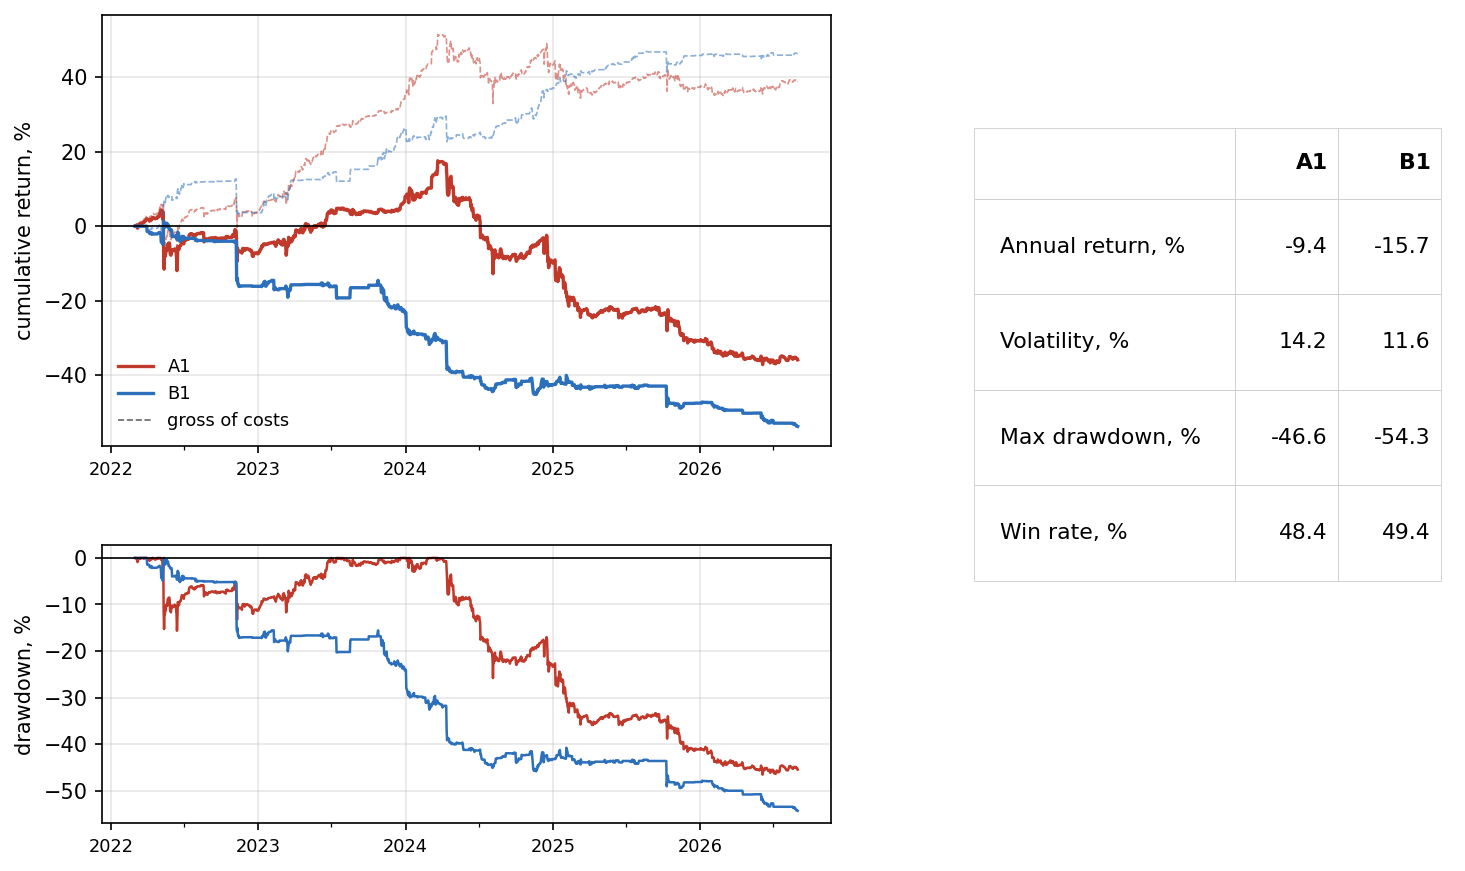
\includegraphics[width=0.92\linewidth,height=0.40\textheight,keepaspectratio]{figs/r3_equity.png}
\caption{Cumulative return net of the 20 bp round trip (solid) and gross of it (dashed), over the underwater curve. Right: portfolio-level statistics, with per-trade numbers in Table 2.}
\end{figure}

The figure puts the same result in the usual form. A1 loses 9.4\% of its capital a year on 14.2\% volatility with a 47\% maximum drawdown; B1 loses 15.7\% on 11.6\% with 54\%. Gross return ends at +39\% and +46\%, net at $-$36\% and $-$54\%, and the gap between the two lines is the round trip, charged 20,602 and 36,047 times. Win rates say the same thing from the other side: gross of costs the two arms win 51.9\% and 55.9\% of trades, and the 20 bp charge takes both below half, because the median gross trade is 10 to 18 bp.

\begin{figure}[H]
\centering
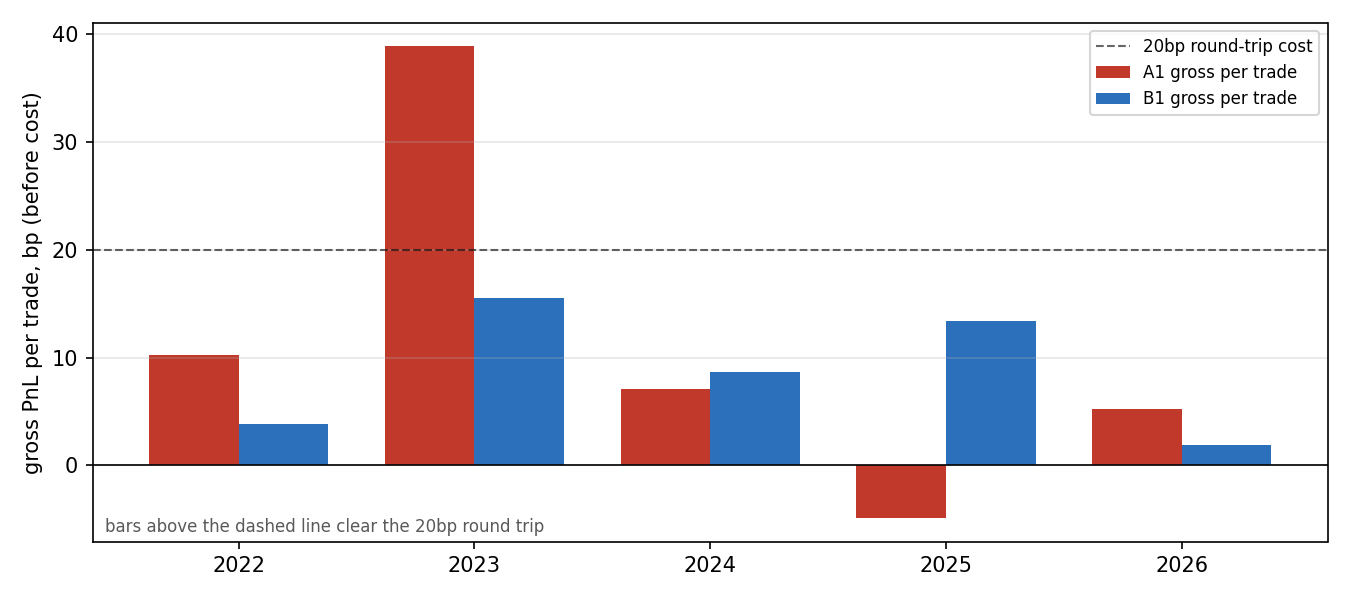
\includegraphics[width=0.92\linewidth,height=0.40\textheight,keepaspectratio]{figs/r3_year.png}
\caption{Gross PnL per trade by year, both strategies, against the 20 bp cost line. Bars above the dashed line would have covered the round trip.}
\end{figure}

The yearly view explains why: A1's gross edge is positive in four of the five years, so it passes the sign test in G4, but it clears the cost line only in 2023, at 38.5 bp per trade, and loses 7.9 bp in 2025. A rule fitted on the full sample cannot trade 2023 in advance.

\subsection{Why the raw numbers mislead}

Raw forward returns measure the market as much as the signal. Across the four cells the raw means at twenty-four hours run from +4.11 to +24.96 bp, because the sample period contains a rising market, while the market-neutral means are negative. R4 with negative funding at eight hours shows the mechanism in one cell: raw +17.86 bp, market-neutral +2.94 bp, with the 14.92 bp between them being the drift.

\section{Conclusion}

The question was whether price and open interest together describe regimes with tradable return information. In this market, at this frequency, they do not. The direction of the next hours has no stable sign: 6 of the 16 increments are significant when every event-hour counts equally, two positive and four negative, and the sign reverses in every cell when every contract-day counts once, with R1 and R4 turning negative. A portfolio built from the labels loses money at every horizon, and the two cells that clear the gates earn 10.38 and 9.26 bp gross against a 20 bp round trip.

What the labels do describe is the size of the next move. All 16 cell-horizon increments in forward volatility are positive and survive correction and the removal of the five most influential contracts; the funding-conditioned replication keeps 83 of 96 contrasts, every one positive, from +6.1\% for negative funding to +17.6\% for extreme. Both tails sit above the neutral middle, so what matters is distance from neutral rather than the sign of the rate. That is an input to sizing and risk budgets, not a directional arm.

\textbf{Contributions.}

\begin{enumerate}
\item A reproducible framework that reads a positioning signal on two margins: the contrast against a same-direction benchmark, which says whether the conditioning adds information, and the level, which says whether a position would earn a return. The gates were fixed before the strategies were priced, and the framework is the transferable part: it would reject most retail signals on the same evidence.
\item An empirical verdict on a widely used signal: a survivorship-controlled universe, multiple-testing control, an explicit market factor, contrasts held against a same-direction benchmark, and tradability tested against zero after costs.
\item An interactive monitor that exposes the same labels the study used, so the claim can be inspected rather than taken on trust.
\end{enumerate}

\bigskip

\section{Future Development}

The report is in-sample throughout: the design was written after the full sample had been seen, and nothing has been run blind. The data cover one venue, Binance, over four and a half years, which is short for a strategy that trades twelve to twenty-two times a day. Funding states are own-history percentiles; in 57\% of rows the 75th and 90th coincide, so the extreme column mixes two different populations. Execution is a single 20 bp round trip with no impact model. There is also no liquidation feed, which is why the recovery-speed question stays open. The grid is hourly; 4- and 8-hour bars were built but never used.

Future work follows from those limits. A five-minute grid would tighten entry timing and test whether the 20 bp charge is the binding constraint or an artefact of the hourly grid. A funding state built on a cross-sectional rank, or on absolute levels rather than own-history percentiles, would remove the degenerate cells. The same design could be run on a second venue, where open interest is measured independently, to see whether the regime is local or market-wide.

The next step is an out-of-sample test. Freeze the design as it stands, wait for data that post-date the sample, and run it once, blind. Only that can say whether the volatility result survives contact with new data.

\bigskip

\section{Self Reflection}

This research broke my unrealistic fantasies and taught me how to test an idea through rigorous experiments. I began with the assumption that clean data and a defensible estimator would eventually produce a signal that could actually make money in the crypto market. However, the direction result is smaller than the cost of trading it and changes sign when the unit of observation switches from the hour to the day. What survives is forward volatility, at every cell and horizon. That is a real result, useful for sizing and risk control, and it is not a trading strategy. Learning to write down why something fails, in a form another person can check, took longer than learning to look for things that pass. The second lesson is about evidence: I used to report the best cell in a table, and I now report the funnel that removed the other ninety-four, because a result that appears at one horizon, under one weighting and in one funding bucket is a choice rather than a finding.

I also made some mistakes during the research process. My first plan was a single universe: rank contracts by liquidity at the end of the sample, take the top fifty, and hold that list for the whole period. That is survivorship bias in its purest form. A contract that stopped trading in 2023 because it had lost its liquidity never enters the list, so the sample keeps only the contracts that made it to 2026. The measured result is overestimated because failed and delisted contracts are ignored. I rebuilt the universe at every month start on the trailing thirty days of quote volume instead, so a contract contributes only to the months in which it qualified, including the months before it delisted. The change cost a full rebuild of the universe and a rerun of every table downstream. The second error was statistical: in an early pass I read the per-cell p-values as the result. Declaring the families and applying Benjamini--Hochberg removed most of them, and the two Phase 4 contrasts that survived correction lost significance when the weighting changed.

If I ran this again I would fix the gate thresholds in a file the analysis reads before I look at any outcome, so that changing a number means rerunning rather than rewriting prose; and I would start from a finer grid, where the 20 bp round trip and the 9 to 10 bp edge are measured at the same frequency.

\bigskip

\section{Acknowledgement}

I thank Professor Wu Xixin for supervision throughout the project, and Mr. Jackson Wong and Mr. Gordon Mak at Theo Quant for the original problem statement. Market data were obtained from Binance's public endpoints.

\textbf{Use of AI tools.} I acknowledge the use of DeepSeek Harness, an AI coding and writing assistant built on DeepSeek models (deepseek v4.1 flash), for the following support: drafting the prose of this report; writing and debugging the analysis code; checking numerical claims against the analysis outputs. The research question, the design of the experiments, the choice of gates and the interpretation of every result are my own. All numbers in this report come from the analysis code rather than from the AI tool, and every figure and table is produced by that code from the data, not by the tool.

\bigskip

\section{Appendices}

\subsection*{Appendix A --- References}

{\small\raggedright\setlength{\parskip}{0.5em}
\noindent\hangindent=1.4em\hangafter=1 Brauneis, A., Mestel, R., Riordan, R., \& Theissen, E. (2021). How to measure the liquidity of cryptocurrency markets? \emph{Journal of Banking \& Finance, 124}, 106041. \url{https://doi.org/10.1016/j.jbankfin.2020.106041}

\noindent\hangindent=1.4em\hangafter=1 Cameron, A. C., Gelbach, J. B., \& Miller, D. L. (2011). Robust inference with multiway clustering. \emph{Journal of Business \& Economic Statistics, 29}(2), 238--249. \url{https://doi.org/10.1198/jbes.2010.07136}

\noindent\hangindent=1.4em\hangafter=1 Christensen, K., Siggaard, M., \& Veliyev, B. (2023). A machine learning approach to volatility forecasting. \emph{Journal of Financial Econometrics, 21}(5), 1680--1727. \url{https://doi.org/10.1093/jjfinec/nbac020}

\noindent\hangindent=1.4em\hangafter=1 Giagkiozis, I., \& Said, E. (2024). Reconciling open interest with traded volume in perpetual swaps. \emph{Ledger, 9}, 1--15. \url{https://doi.org/10.5195/ledger.2024.325}

\noindent\hangindent=1.4em\hangafter=1 Harvey, C. R., \& Liu, Y. (2020). False (and missed) discoveries in financial economics. \emph{Journal of Finance, 75}(5), 2503--2553. \url{https://doi.org/10.1111/jofi.12951}

\noindent\hangindent=1.4em\hangafter=1 He, S., Manela, A., Ross, O., \& von Wachter, V. (2022). \emph{Fundamentals of perpetual futures} (arXiv:2212.06888). \url{https://arxiv.org/abs/2212.06888}

\noindent\hangindent=1.4em\hangafter=1 Hou, K., Xue, C., \& Zhang, L. (2020). Replicating anomalies. \emph{Review of Financial Studies, 33}(5), 2019--2133. \url{https://doi.org/10.1093/rfs/hhy131}

\noindent\hangindent=1.4em\hangafter=1 Jadouli, A. (2026). \emph{Predictive extrema, unprofitable policies: An AI-assisted audit of candle-based Binance spot timing models} (arXiv:2607.19453). \url{https://arxiv.org/abs/2607.19453}

\noindent\hangindent=1.4em\hangafter=1 Jensen, T. I., Kelly, B., \& Pedersen, L. H. (2023). Is there a replication crisis in finance? \emph{Journal of Finance, 78}(5), 2465--2518. \url{https://doi.org/10.1111/jofi.13249}

\noindent\hangindent=1.4em\hangafter=1 Kim, D.-H. (2026). Perpetual futures as predictors of Bitcoin volatility. \emph{Journal of Empirical Finance, 89}, 101779. \url{https://doi.org/10.1016/j.jempfin.2026.101779}

\noindent\hangindent=1.4em\hangafter=1 Naredla, V. (2026). \emph{Path signatures for regime detection in cryptocurrency markets: A rough-path framework using spot, perpetual basis, and funding rates} [SSRN working paper]. \url{https://doi.org/10.2139/ssrn.6609698}

\noindent\hangindent=1.4em\hangafter=1 Petersen, M. A. (2009). Estimating standard errors in finance panel data sets: Comparing approaches. \emph{Review of Financial Studies, 22}(1), 435--480. \url{https://doi.org/10.1093/rfs/hhn053}

\noindent\hangindent=1.4em\hangafter=1 Seo, S. W., Byun, S. J., \& Kim, J. S. (2020). Index options open interest and stock market returns. \emph{Journal of Futures Markets, 40}(6), 989--1010. \url{https://doi.org/10.1002/fut.22095}

\noindent\hangindent=1.4em\hangafter=1 Zaremba, A., Bilgin, M. H., Long, H., Mercik, A., \& Szczygielski, J. J. (2021). Up or down? Short-term reversal, momentum, and liquidity effects in cryptocurrency markets. \emph{International Review of Financial Analysis, 78}, 101908. \url{https://doi.org/10.1016/j.irfa.2021.101908}

\noindent\hangindent=1.4em\hangafter=1 DeepSeek. (2026). \emph{DeepSeek Harness} (accessed 24 November 2026). \url{https://www.deepseek.com}

\subsection*{Appendix B --- List of Figures and Tables}

{\footnotesize\setlength{\tabcolsep}{4pt}
\begin{longtable}{p{0.15\linewidth}p{0.40\linewidth}p{0.15\linewidth}p{0.20\linewidth}}
\toprule
Item & Caption & Section & Source \\
\midrule
\endfirsthead
\toprule
Item & Caption & Section & Source \\
\midrule
\endhead
\bottomrule
\endfoot
Figure 1 & Coverage by month, four sources & 4.3 & figs/q1\_coverage.png \\
Figure 2 & Threshold sensitivity of the four labels & 4.3 & figs/q2\_threshold.png \\
Figure 3 & Master table of the board & 5.4 & figs/d5\_master.png \\
Figure 4 & The four directional lists & 5.4 & figs/d5\_events.png \\
Figure 5 & Funding-adjusted crowding & 5.4 & figs/d5\_crowding.png \\
Figure 6 & Realised volatility panel & 5.4 & figs/d5\_vol.png \\
Figure 7 & Forward volatility by cell and horizon & 6.1 & figs/r1\_volatility.png \\
Figure 8 & Mean forward return against the benchmark & 6.1 & figs/r1\_direction.png \\
Figure 9 & Return by weighting and within-day persistence & 6.1 & figs/r1\_weighting.png \\
Figure 10 & Price-by-open-interest interaction & 6.1 & figs/r1\_interaction.png \\
Figure 11 & Reversal rate and its gap to the benchmark & 6.1 & figs/r1\_reversal.png \\
Figure 12 & Four-state minus each single-signal baseline & 6.2 & figs/r2\_baselines.png \\
Figure 13 & Placebo against random timing & 6.2 & figs/r2\_placebo.png \\
Figure 14 & Funding contrasts at every horizon & 6.3 & figs/r2\_panorama.png \\
Figure 15 & Cumulative PnL and drawdown & 6.4 & figs/r3\_equity.png \\
Figure 16 & Gross PnL per trade by year & 6.4 & figs/r3\_year.png \\
Figure 17 & Full board, screen layout & App. C & figs/d5\_full.png \\
Table 1 & Forward return by cell and horizon, market-neutral & 6.1 &  \\
Table 2 & The two surviving strategies, net of cost & 6.4 &  \\
\end{longtable}
}

\subsection*{Appendix C --- Screen layouts}

\begin{figure}[H]
\centering
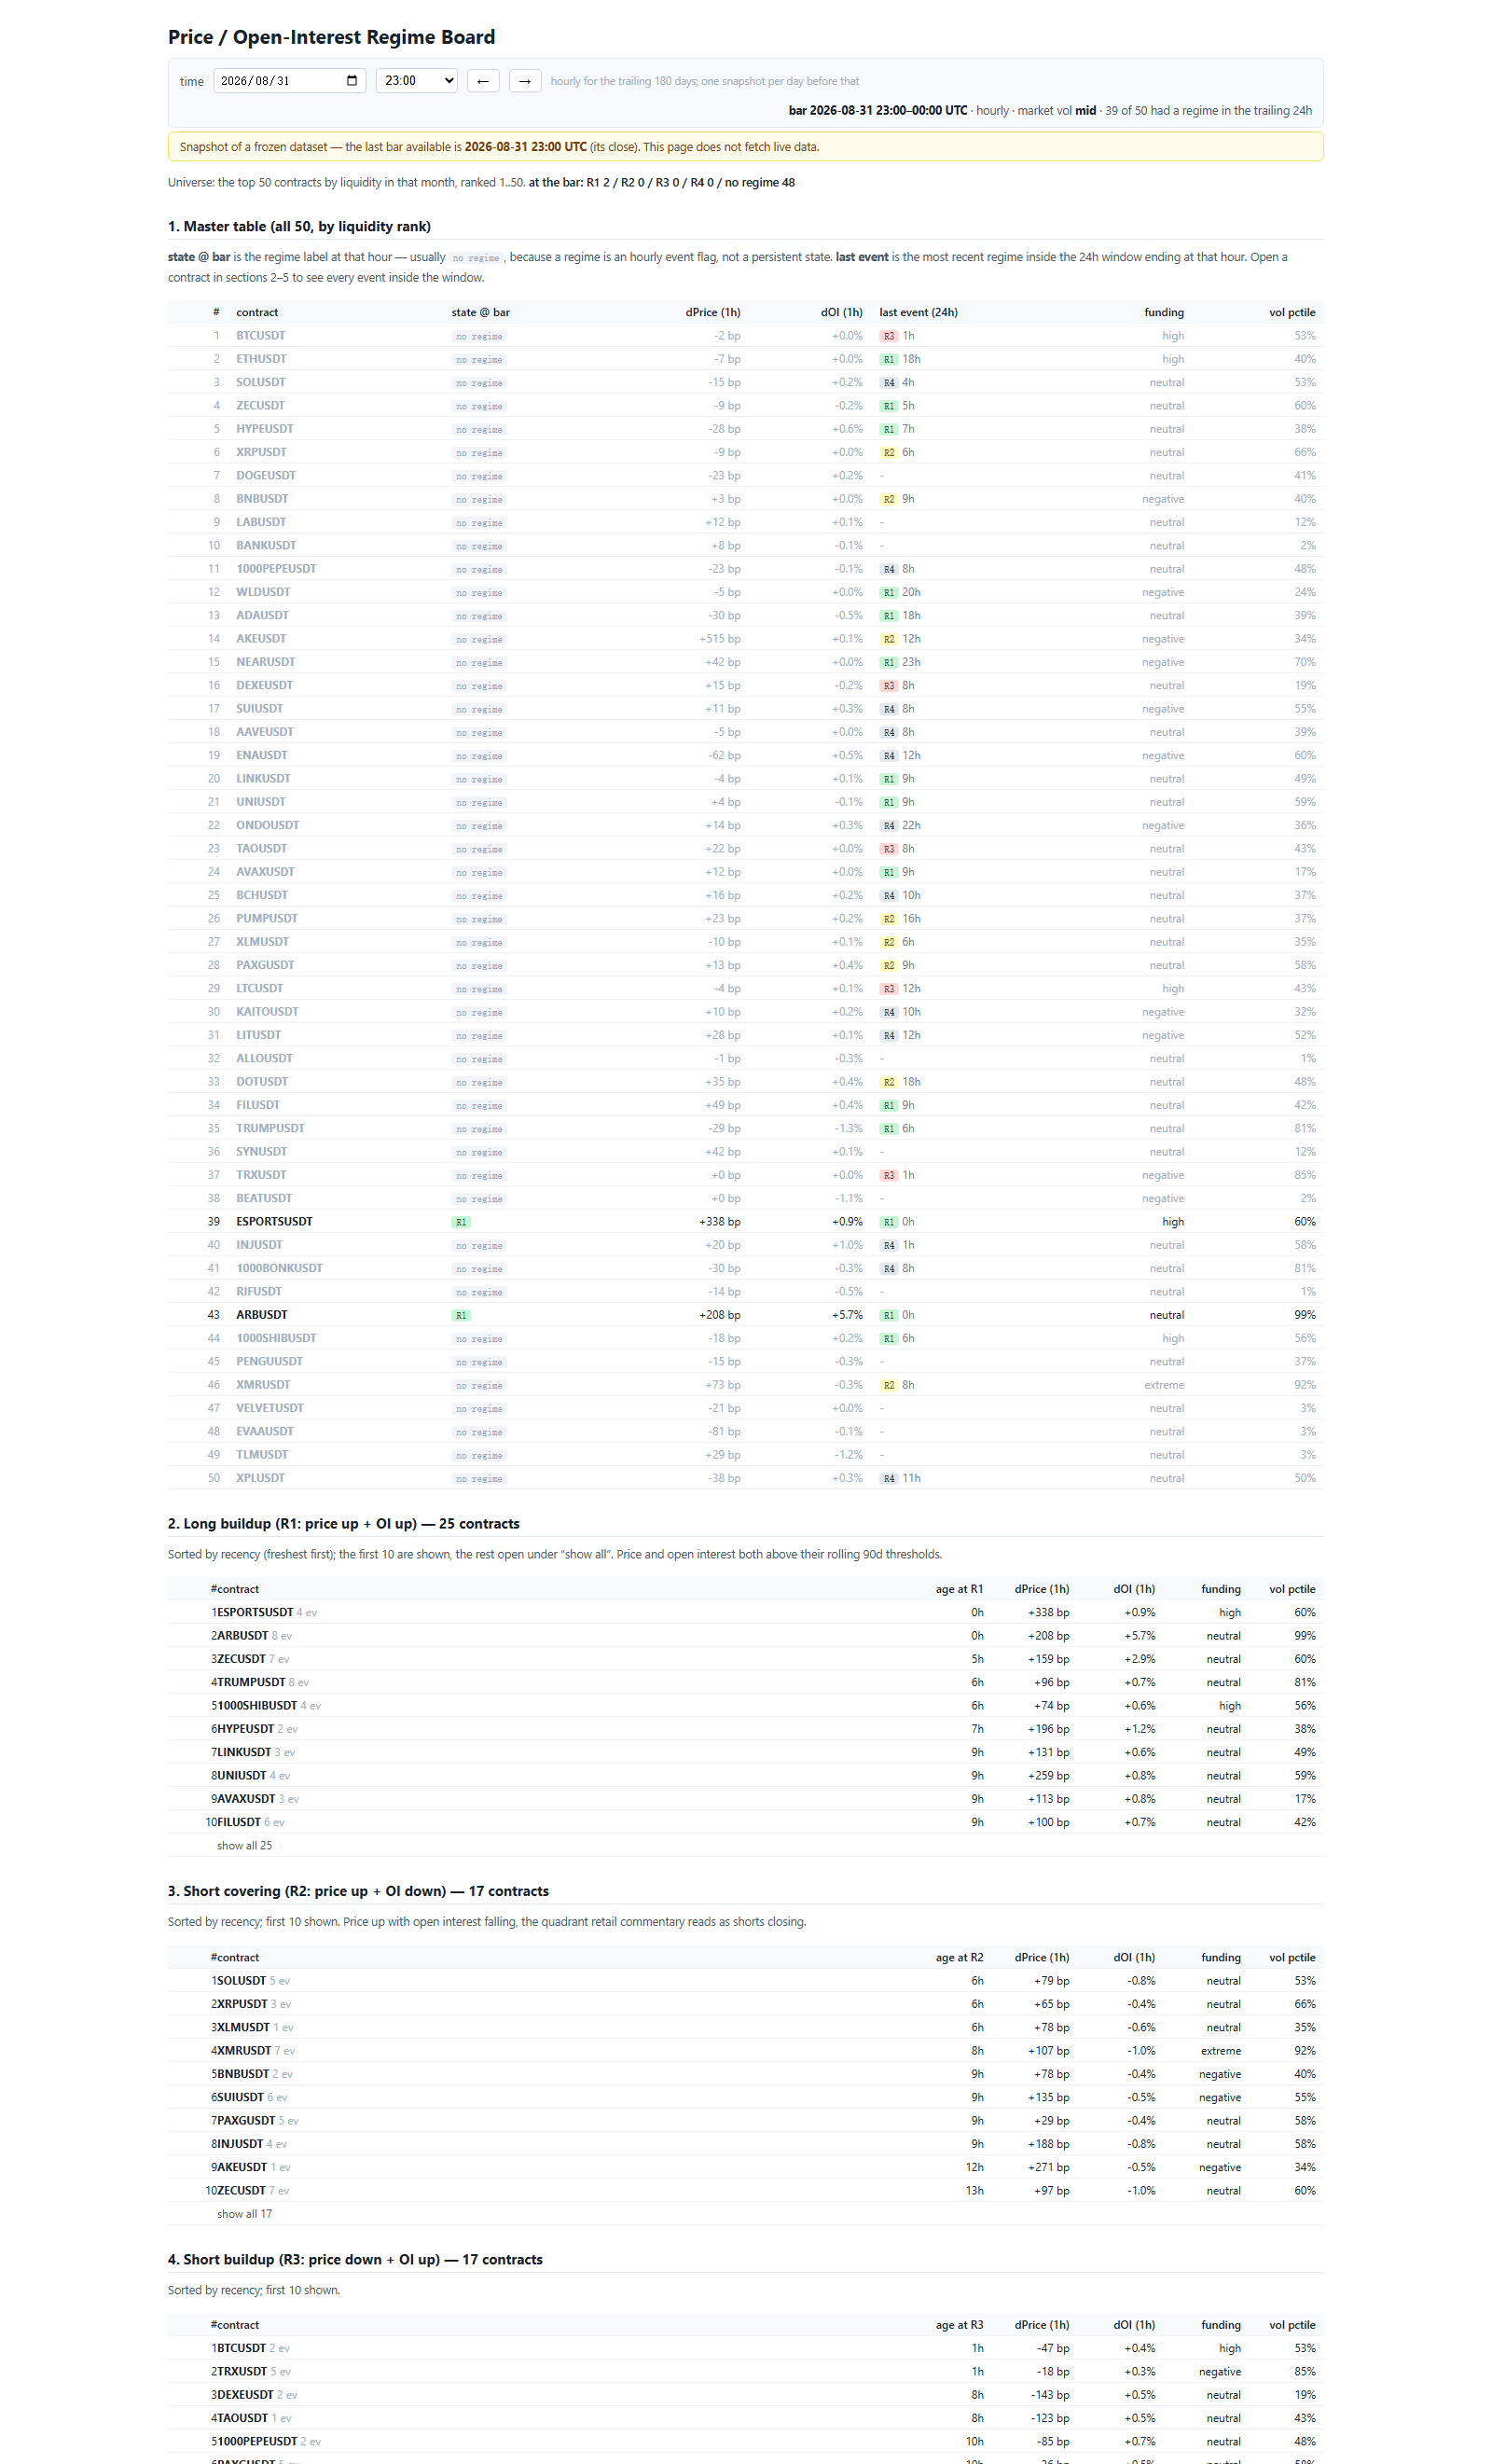
\includegraphics[width=\linewidth,height=0.90\textheight,keepaspectratio]{figs/d5_full_p1.png}
\caption*{Figure 17. The full board, 2026-08-31 23:00 UTC, rendered at 1600 px and reduced to fit the page: seven sections, from the master table through the four lists, the crowding view and realised volatility. (1 of 2)}
\end{figure}

\begin{figure}[H]
\centering
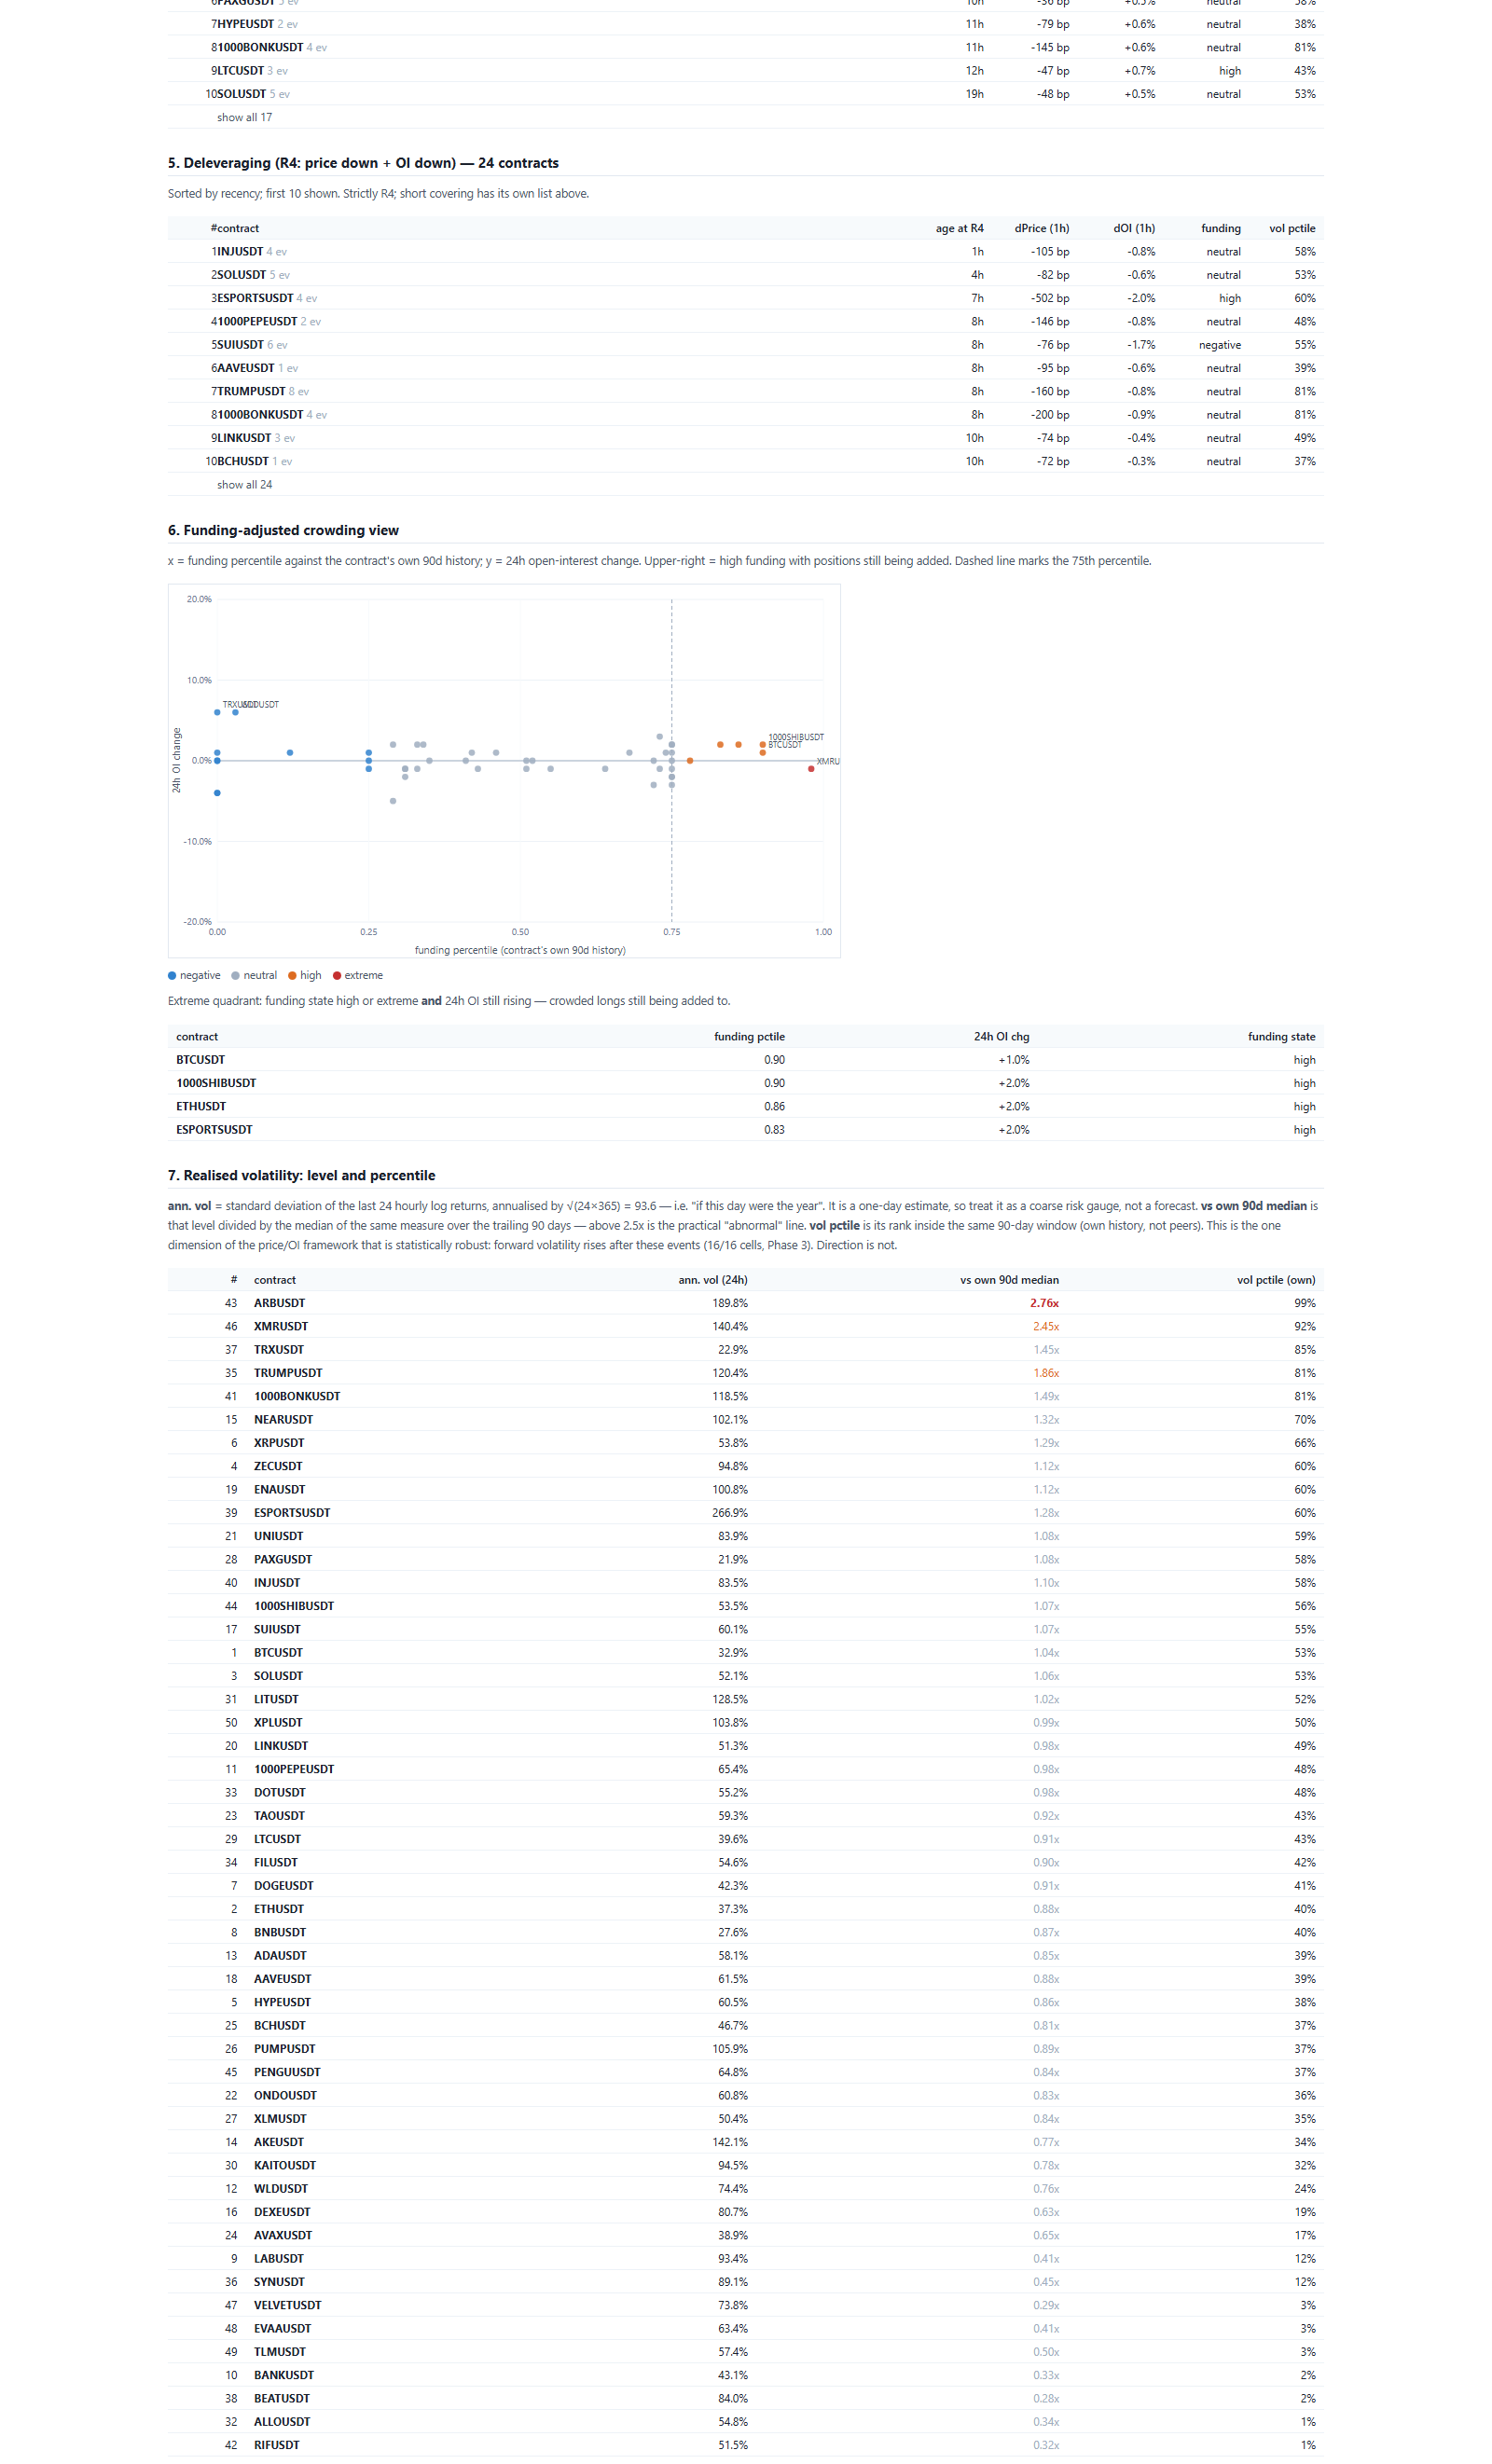
\includegraphics[width=\linewidth,height=0.90\textheight,keepaspectratio]{figs/d5_full_p2.png}
\caption*{Figure 17. The full board, 2026-08-31 23:00 UTC, rendered at 1600 px and reduced to fit the page: seven sections, from the master table through the four lists, the crowding view and realised volatility. (2 of 2)}
\end{figure}

\subsection*{Appendix D --- Sample construction}

Every row below is a filter on the hourly grid, and each one removes a different kind of observation.

\begin{table}[H]\centering
\footnotesize
\begin{tabularx}{\linewidth}{>{\raggedright\arraybackslash}X>{\raggedright\arraybackslash}X>{\raggedright\arraybackslash}X}
\toprule
Stage & Units & What it means \\
\midrule
Hourly grid & 7,253,002 rows, 285 contracts, 57 months & one row per contract-hour; a missing bar stays as a row and is flagged, not dropped \\
Labelled panel & 7,252,717 rows, 41,639 hours, 174 contracts an hour & one row fewer per contract, because the last bar has no next bar to price a forward return \\
Labelled events & 923,235 rows, 12.7\% of the grid & both changes above their own trailing 90-day p70 \\
Universe & 2,700 contract-months, 249 contracts, 54 months & 50 contracts a month, four gates and a ranking (below); 54 rather than 57 months because the first three lack history \\
Headline sample & 256,079 events & in universe, exclusion flag ok, cell 1 to 4 \\
With a 1-hour forward & 256,076 events & three events have no forward price \\
With a funding state & 255,857 events & 219 events, 0.09\%, have no percentile defined \\
Funding settlements & 1,229,941 & 8-hour 52\%, 4-hour 45\%, 1-hour 3\% of settlements, 0.1\% on a two-hour schedule \\
\bottomrule
\end{tabularx}
\end{table}

The universe is rebuilt at every month start, and a contract has to pass four gates before it is ranked.

\begin{table}[H]\centering
\footnotesize
\begin{tabularx}{\linewidth}{>{\raggedleft\arraybackslash}X>{\raggedright\arraybackslash}X>{\raggedright\arraybackslash}X}
\toprule
Gate & Rule & Threshold in this study \\
\midrule
1 & the base asset is not a stablecoin or a fiat currency & 11 bases (USDC, FDUSD, TUSD, BUSD, DAI, USDP, SUSD, USDD, PYUSD, FRAX, USTC), judged on the base asset rather than the ticker \\
2 & enough history, and still trading & 2,160 hourly bars (90 days) by the month start, and a last active date no earlier than that start \\
3 & open interest is present and continuous & coverage of at least 90\% of all hours in the trailing 30 days, and no publication gap longer than 48 hours \\
4 & the contract is a crypto perpetual & contract type PERPETUAL with underlying COIN; tokenised equities, ETFs and FX are excluded, while PAXG and XAUT are kept because they trade around the clock \\
\bottomrule
\end{tabularx}
\end{table}

Liquidity enters as a ranking: contracts that pass all four are ordered by the median quote volume of the trailing 30 days, and the top fifty become that month's universe. The window ends at the month start, so no contract is ranked on data from the month it trades in.

\subsection*{Appendix E --- Label robustness}

Both label definitions were varied and the effect on the analysis sample recorded. Neither variation changes the sign of any result in the text.

\textbf{Threshold level.} Moving the event threshold from the 55th to the 80th percentile of each contract's own trailing distribution cuts the labelled share from 23.0\% to 7.5\% at one hour. The mix inside the labelled set is more stable than the count: the largest shift in any regime's share is 1.8 percentage points at p70 and 3.8 points at p80, and 5.5 and 11.8 points at one day.

\begin{table}[H]\centering
\footnotesize
\begin{tabularx}{\linewidth}{>{\raggedright\arraybackslash}X>{\raggedleft\arraybackslash}X>{\raggedleft\arraybackslash}X>{\raggedright\arraybackslash}X>{\raggedright\arraybackslash}X}
\toprule
Threshold & Labelled share, 1h & Labelled share, 1d & Largest mix shift, 1h & Largest mix shift, 1d \\
\midrule
p55 & 23.0\% & 22.9\% & --- & --- \\
p70 (used) & 12.8\% & 12.6\% & 1.8 pp & 5.5 pp \\
p80 & 7.5\% & 7.3\% & 3.8 pp & 11.8 pp \\
\bottomrule
\end{tabularx}
\end{table}

\textbf{Funding labels.} In 57\% of event rows the 75th and 90th percentiles of the contract's funding history fall on the same value, so high and extreme are the same rows. Separating them shows two populations: in R3 at one hour the degenerate bucket averages +4.65 bp against $-$6.94 bp for high-only and $-$0.85 bp for the pooled extreme column. The degenerate bucket is also thin, 217 to 316 contract-months at one hour, which is why the gate merges the two labels rather than testing extreme on its own.

\end{document}
